\title{Energy-profiling Zoleria RE-Mote}

\documentclass[a4paper]{article}

\usepackage[english]{babel}
\usepackage[utf8]{inputenc}
\usepackage{amsmath}
\usepackage{graphicx}
\usepackage{subcaption}
\usepackage{hyperref}
\usepackage[colorinlistoftodos]{todonotes}
\usepackage{float}


\author{Srijith Nair}

\date{\today}

\begin{document}
\maketitle

\begin{abstract}
Energy scavenging motes have a crucial role to play in today's world driven by intelligent IoT networks. Low power devices, commonly called motes, which can sense real-time data, are becoming increasingly popular for IoT applications. The maintenance costs and lifetime of such devices depends greatly on their power consumption. It is therefore essential to measure the power consumption of the motes before deciding on which energy-harvesting techniques to use for powering them. This report shows the fundamentals of how to measure the energy consumption of one such mote, Zolertia RE-Mote, under different modes and scenarios of operation.
\end{abstract}

\section{Introduction}
\label{sec:introduction}
The Internet of Things (IoT) has been gaining wide popularity in both industry and research fronts in the past few years. The idea of accessing any device via the Internet is now taking its shape in reality. This has driven research in multiple fronts, to steer towards this common goal. Network engineering is now focusing on creating network topologies and optimal protocols to maintain reliable communication among devices in such networks. Electronics engineering has become focused at creating low-power wireless devices which are capable of sensing and actuating coordinated tasks based on application. Computer scientists and engineers are now working on developing reliable cloud, edge and fog computing algorithms to optimally control such networks.

IoT Networks are constructed keeping in mind scalability among many other parameters. For networks to scale, it is important to take into account the power consumed by it's motes. The power consumed by individual motes is almost never constant with time. There are a lot of different cases in real-time systems where there may be intermittent surges in the power consumed due to radio power duty-cycling, transmissions, sensor sampling, or even computation. Any long-term project should, thus, account for all these factors before charting out the power budget.

The rest of this report is structured as follows. \textbf{Section 2} consists of a theoretical overview of the Zolertia RE-Mote platform (\textbf{Section 2.1}), the Contiki Operating system (\textbf{Section 2.2}), the Tektronics TCPA300 current probe and amplifier (\textbf{Section 2.3}), and the conversion of current readings into energy (\textbf{Section 2.4}); \textbf{Section 3} presents the experiment performed to take current consumption measurements; \textbf{Section 4} shows some typical results in the form of Current-Time plots; and, \textbf{Section 5} concludes this report.

\section{Theory}
\label{sec:theory}

\subsection{Zolertia RE-Mote}
RE-Mote is a ultra-low power consuming device manufactured by Zolertia for IoT applications. A picture of RE-Mote Rev-B is shown in figure \ref{fig:remote} The platform is powered by a Texas Instruments CC2538 ARM Cortex-M3 system on chip (SoC) \cite{remote}. RE-Mote has support for 2.4GHz and sub-1GHz communication ranges as specified in the IEEE 802.15.4 standards \cite{ieee802154}. The IEEE 802.15.4 standard provides data rates of upto 250kbps. Support for Zoleria RE-Mote is available in the Contiki Operating System \cite{contiki}.

\begin{figure}
\centering
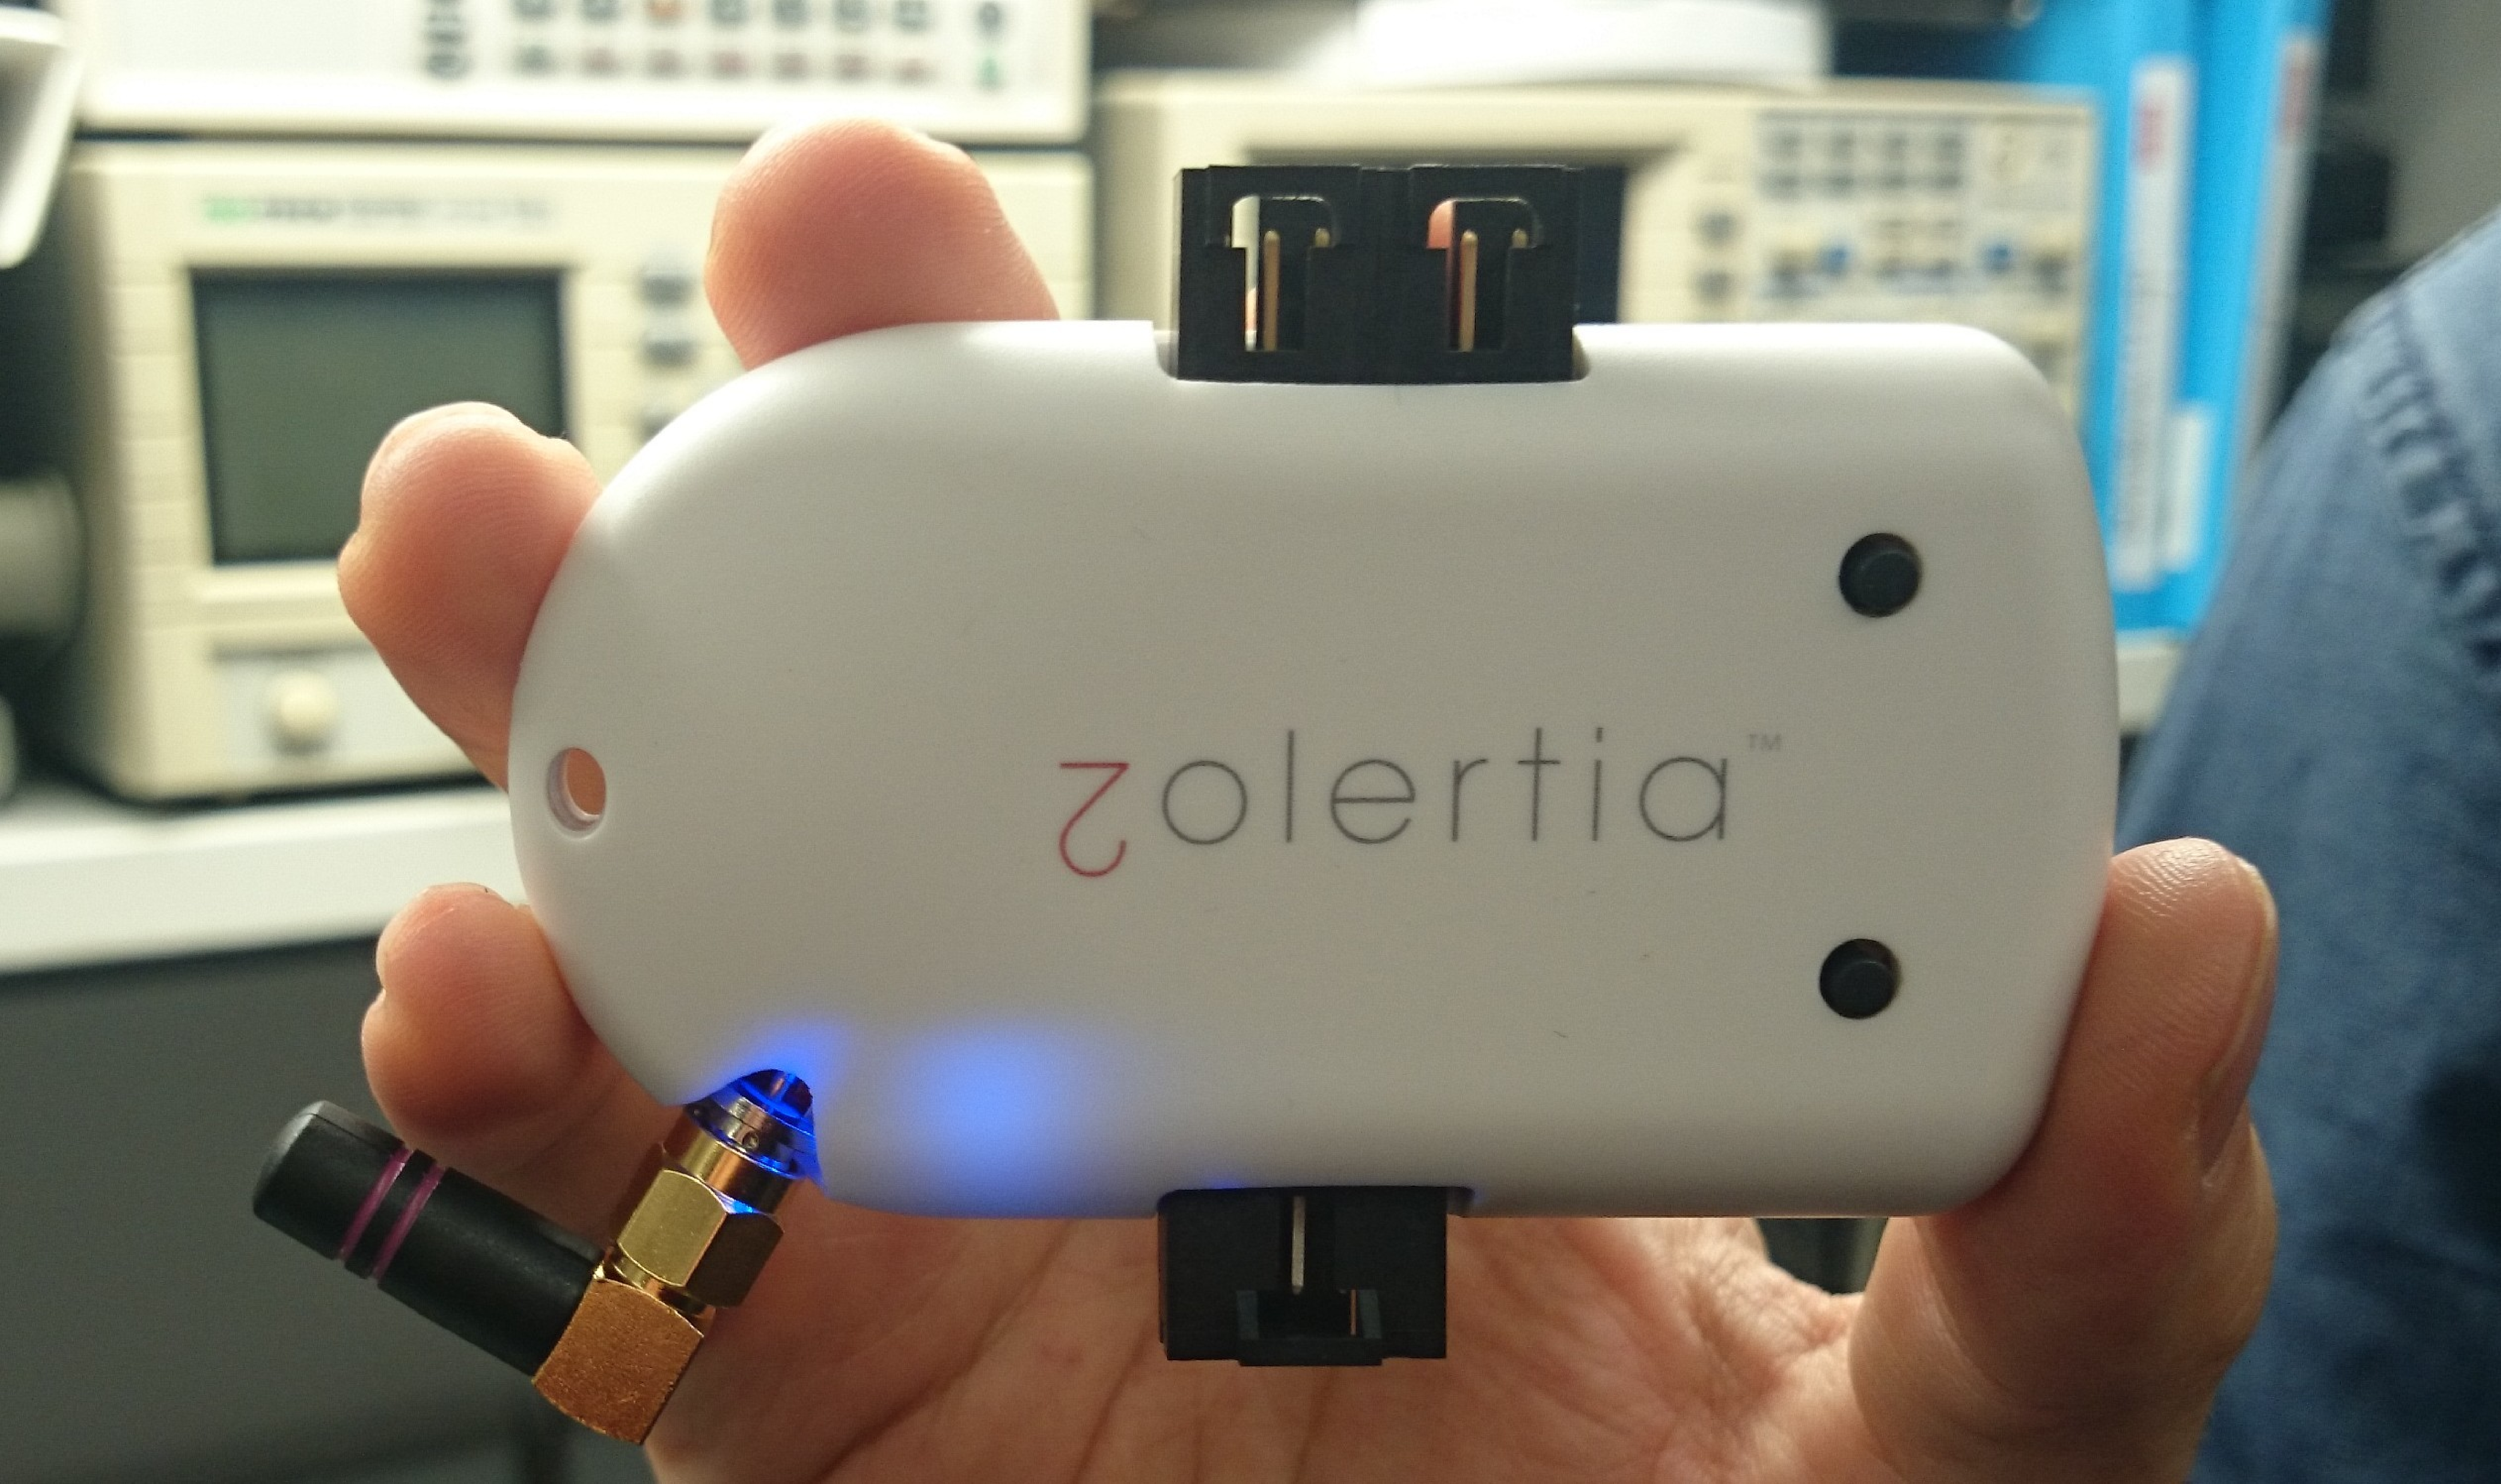
\includegraphics[width=0.7\textwidth]{images/remote.pdf}
\caption{\label{fig:remote}Zolertia RE-Mote Revision-B mote}
\end{figure}

\subsection{Contiki OS}
The Contiki Operating System\cite{contiki} is a lightweight operating system for low power devices. Contiki has open source implementations of many constrained node networking protocols like RPL, 6LoWPAN, CoAP, MQTT and so on. It also has support for various radio drivers like CC1200, CC2538, CC2420, etc. Zolertia RE-Motes can work with CC1200 driver (for sub-1GHz operation) and with CC2538 driver (for 2.4GHz operation). Since both these drivers have stable implementations in Contiki OS, it makes it a suitable OS for running on RE-Mote.

Constrained devices need optimized resource management for operting on battery power for long durations (typically years). The radio transievers are found to consume the most power in a low-power device. Contiki has a Radio Duty-Cycling protocol called ContikiMAC \cite{contikimac} which has a scheme for switching off the radio for $99\%$ of the time. This saves a lot of power. The plot in figure \ref{fig:revb-rdcs} shows the difference in the power consumed with and without duty-cycling in RE-Mote Revision B.

%\begin{figure}
%\centering
%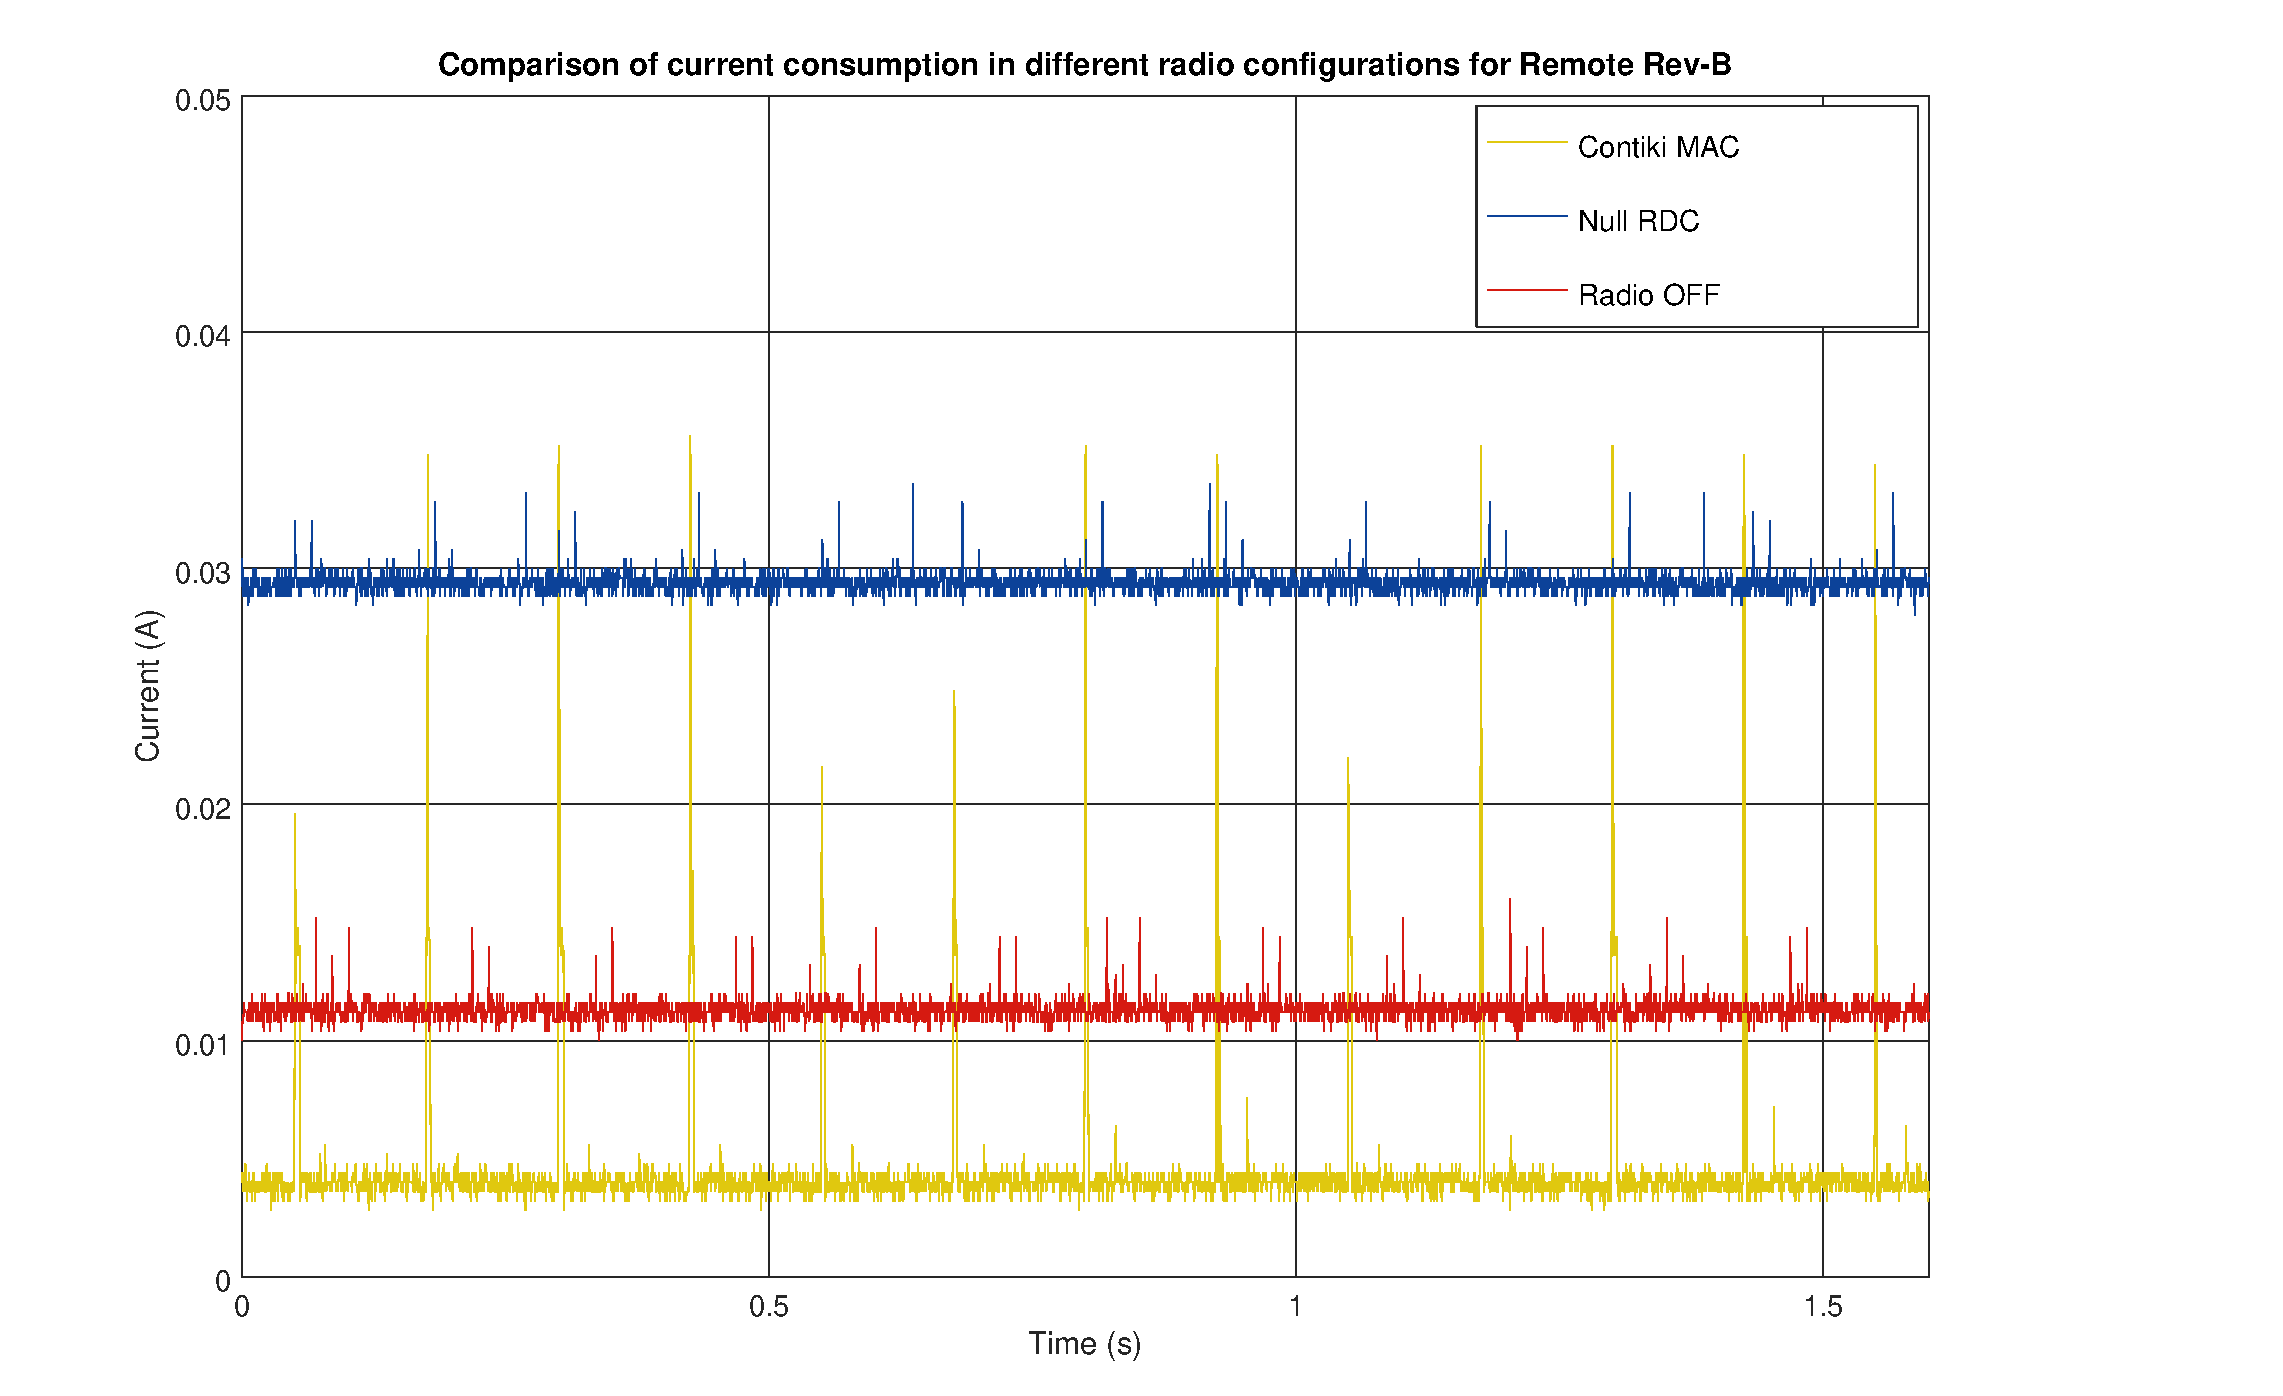
\includegraphics[width=1\textwidth]{plots/revb-rdc.eps}
%\caption{\label{fig:revbrdc}Tektronics TCPA300 Current Probe and Amplifier}
%\end{figure}

\subsection{Tektronics TCPA300 current probe}
A current probe is a device that measures current in a wire by converting it to a proportional change in voltage. It works on the principle of Hall effect and is thus called a Hall-effect device. The probe consists of a clamp that loops around the wire to measure current. A sliding jaw on the clamp makes looping across the wire easy. Figure \ref{fig:probe} shows a TCPA300 current probe by Tektronics. 

The current amplifier is used to set the calibration and to de-Gauss the current probe. De-Gaussing is an important prerequisite to using the current probe. It involves marking the zero current line to prevent bias in future readings. The TCPA300 current amplifier has an option to Autobalance the zero line.

\begin{figure}
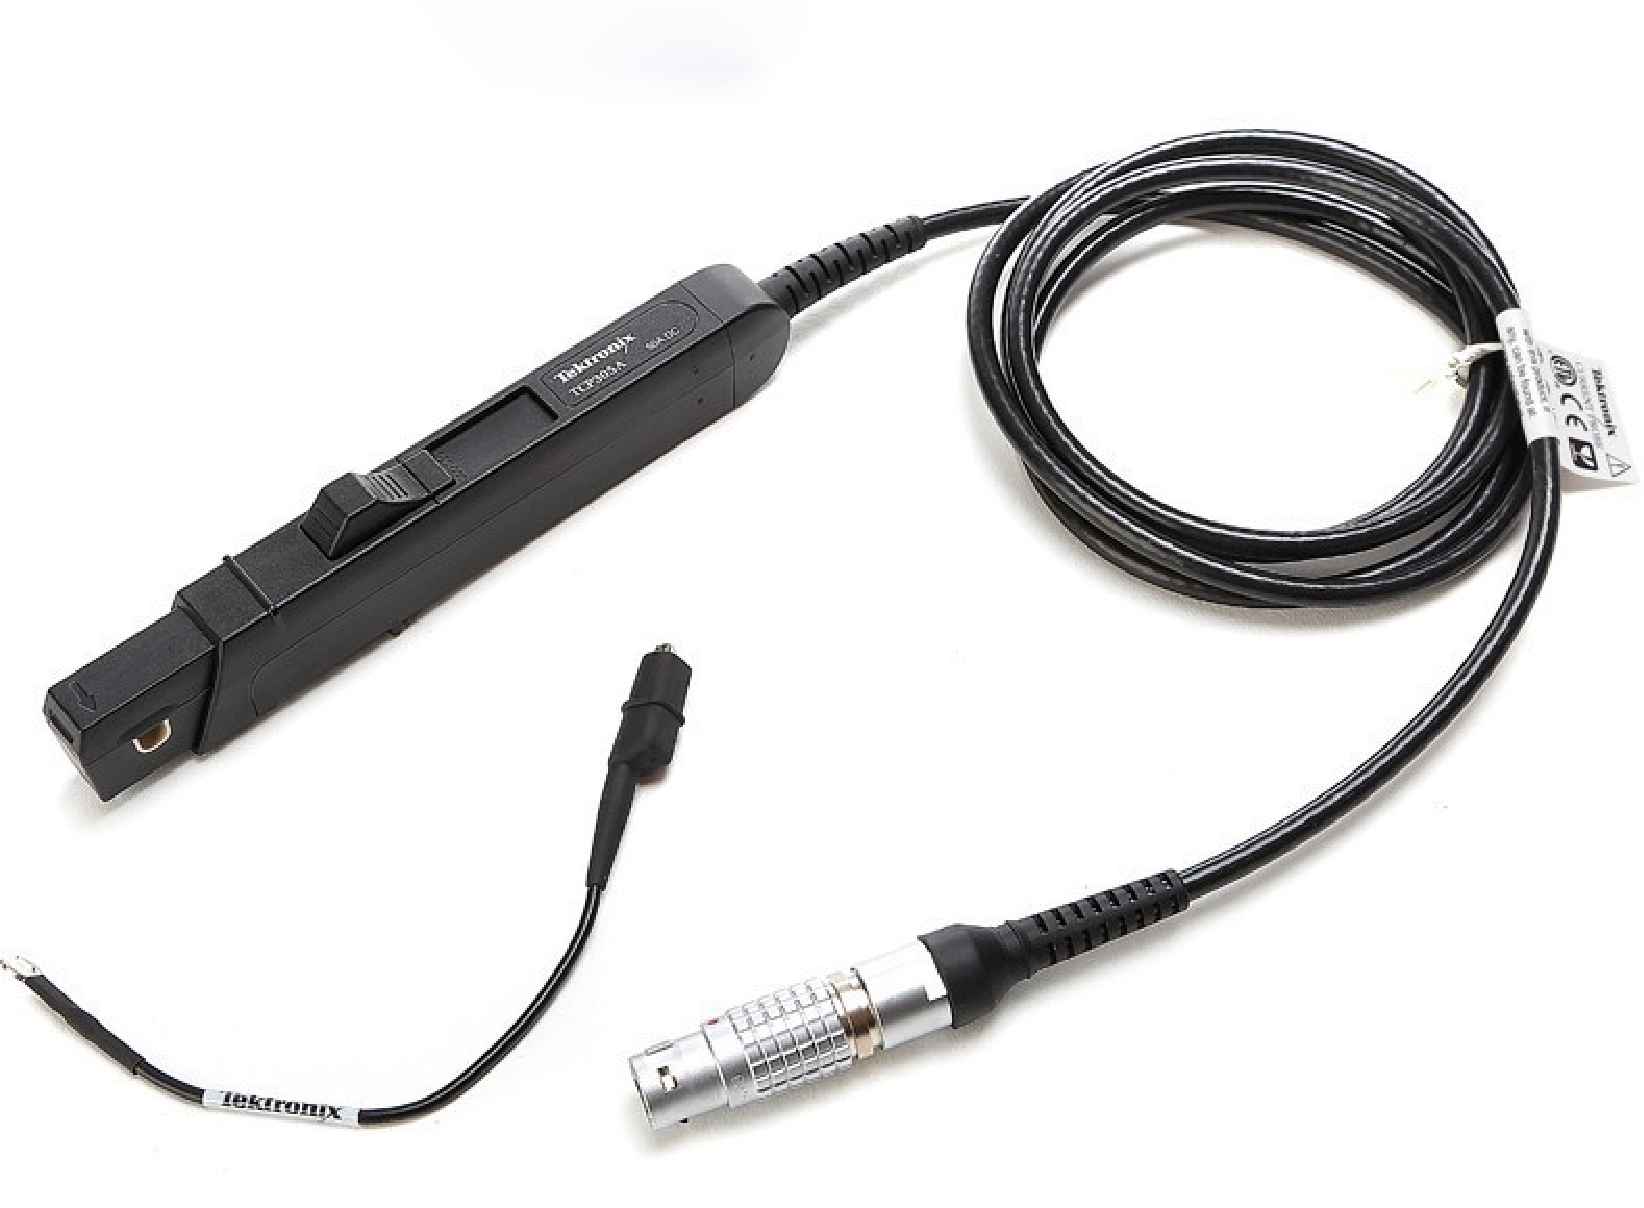
\includegraphics[width=0.5\textwidth]{images/current-probe.pdf}
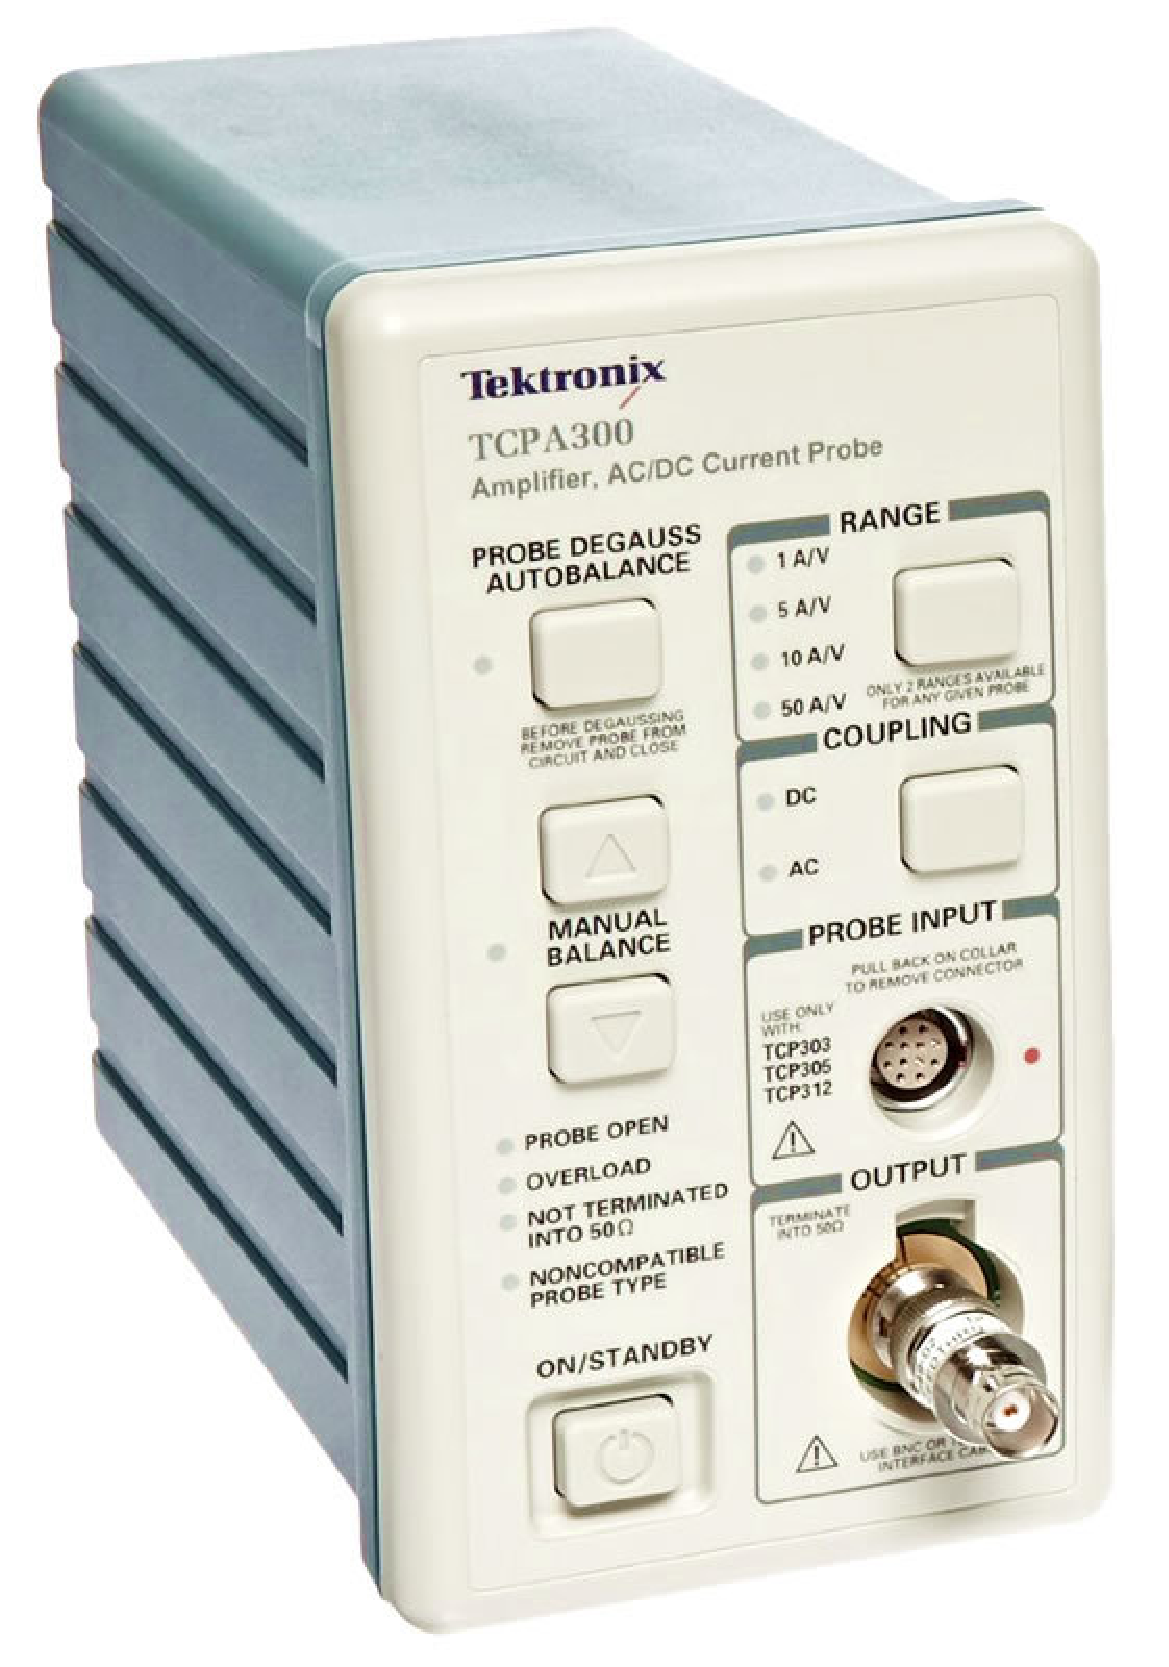
\includegraphics[width=0.4\textwidth]{images/current-amp.pdf}
\caption{\label{fig:probe}Tektronics TCPA300 Current Probe and Amplifier}
\end{figure}

\subsection{Conversion of current readings to Energy}
The output on the screen of the DSO, measures current consumed as a function of time. The energy can be theoretically calculated from the sample points thus obtained.\par
From the definition of power, it can be said that,
$$ P(t) = \frac{dE(t)}{dt} $$
Thus $E(t)$ is an integral of $P(t)$
$$ E(t) = \int_{0}^{t}P(t)dt $$
since power is a product of instantaneous voltage and current, and since the voltage is a constant,
$$ P(t) = V \times I(t) $$
$$ E(t) = V \times \int_{0}^{t}I(t)dt $$

Thus, the energy of the RE-Mote device under a certain configuration is the product of the supplied voltage and the area under the current-time curve.

\section{Experiment}

\subsection{Equipment required}
The following equipment is needed before proceeding with the experiment. Any alternatives to the current probe, DSO or the power supply box should work fine.
\begin{enumerate}
	\item{Current measuring probe: Tektronics TCPA300 - 1x}
    \item{Tektronics TCPA300 current amplifier        - 1x}
    \item{Tektronics 5100 series oscilloscope         - 1x}
	\item{Tekprobe interface cable                    - 1x}
	\item{Zolertia RE-Motes (Rev A and Rev B)         - 2x}
	\item{AlphaSense $SO_2$ sensor                    - 1x}
	\item{GWINSTEK GPS-2303 DC power supply box       - 1x}
	\item{Male-Female jumpers                         - 2x}
	\item{Female-Female jumpers                       - 4x}
	\item{Bread board                                 - 1x}
\end{enumerate}

\subsection{Experimental set-up}
The experimental set-up is as shown in the block diagram in Figure \ref{fig:circuit}. A power-supply box is adjusted to provide not more than 3.4V. Pin-outs of Rev A and Rev B are shown for easy reference in Figures \ref{fig:revapins} and \ref{fig:revbpins}.


\begin{figure}
\begin{minipage}{0.5\textwidth}
  \centering
  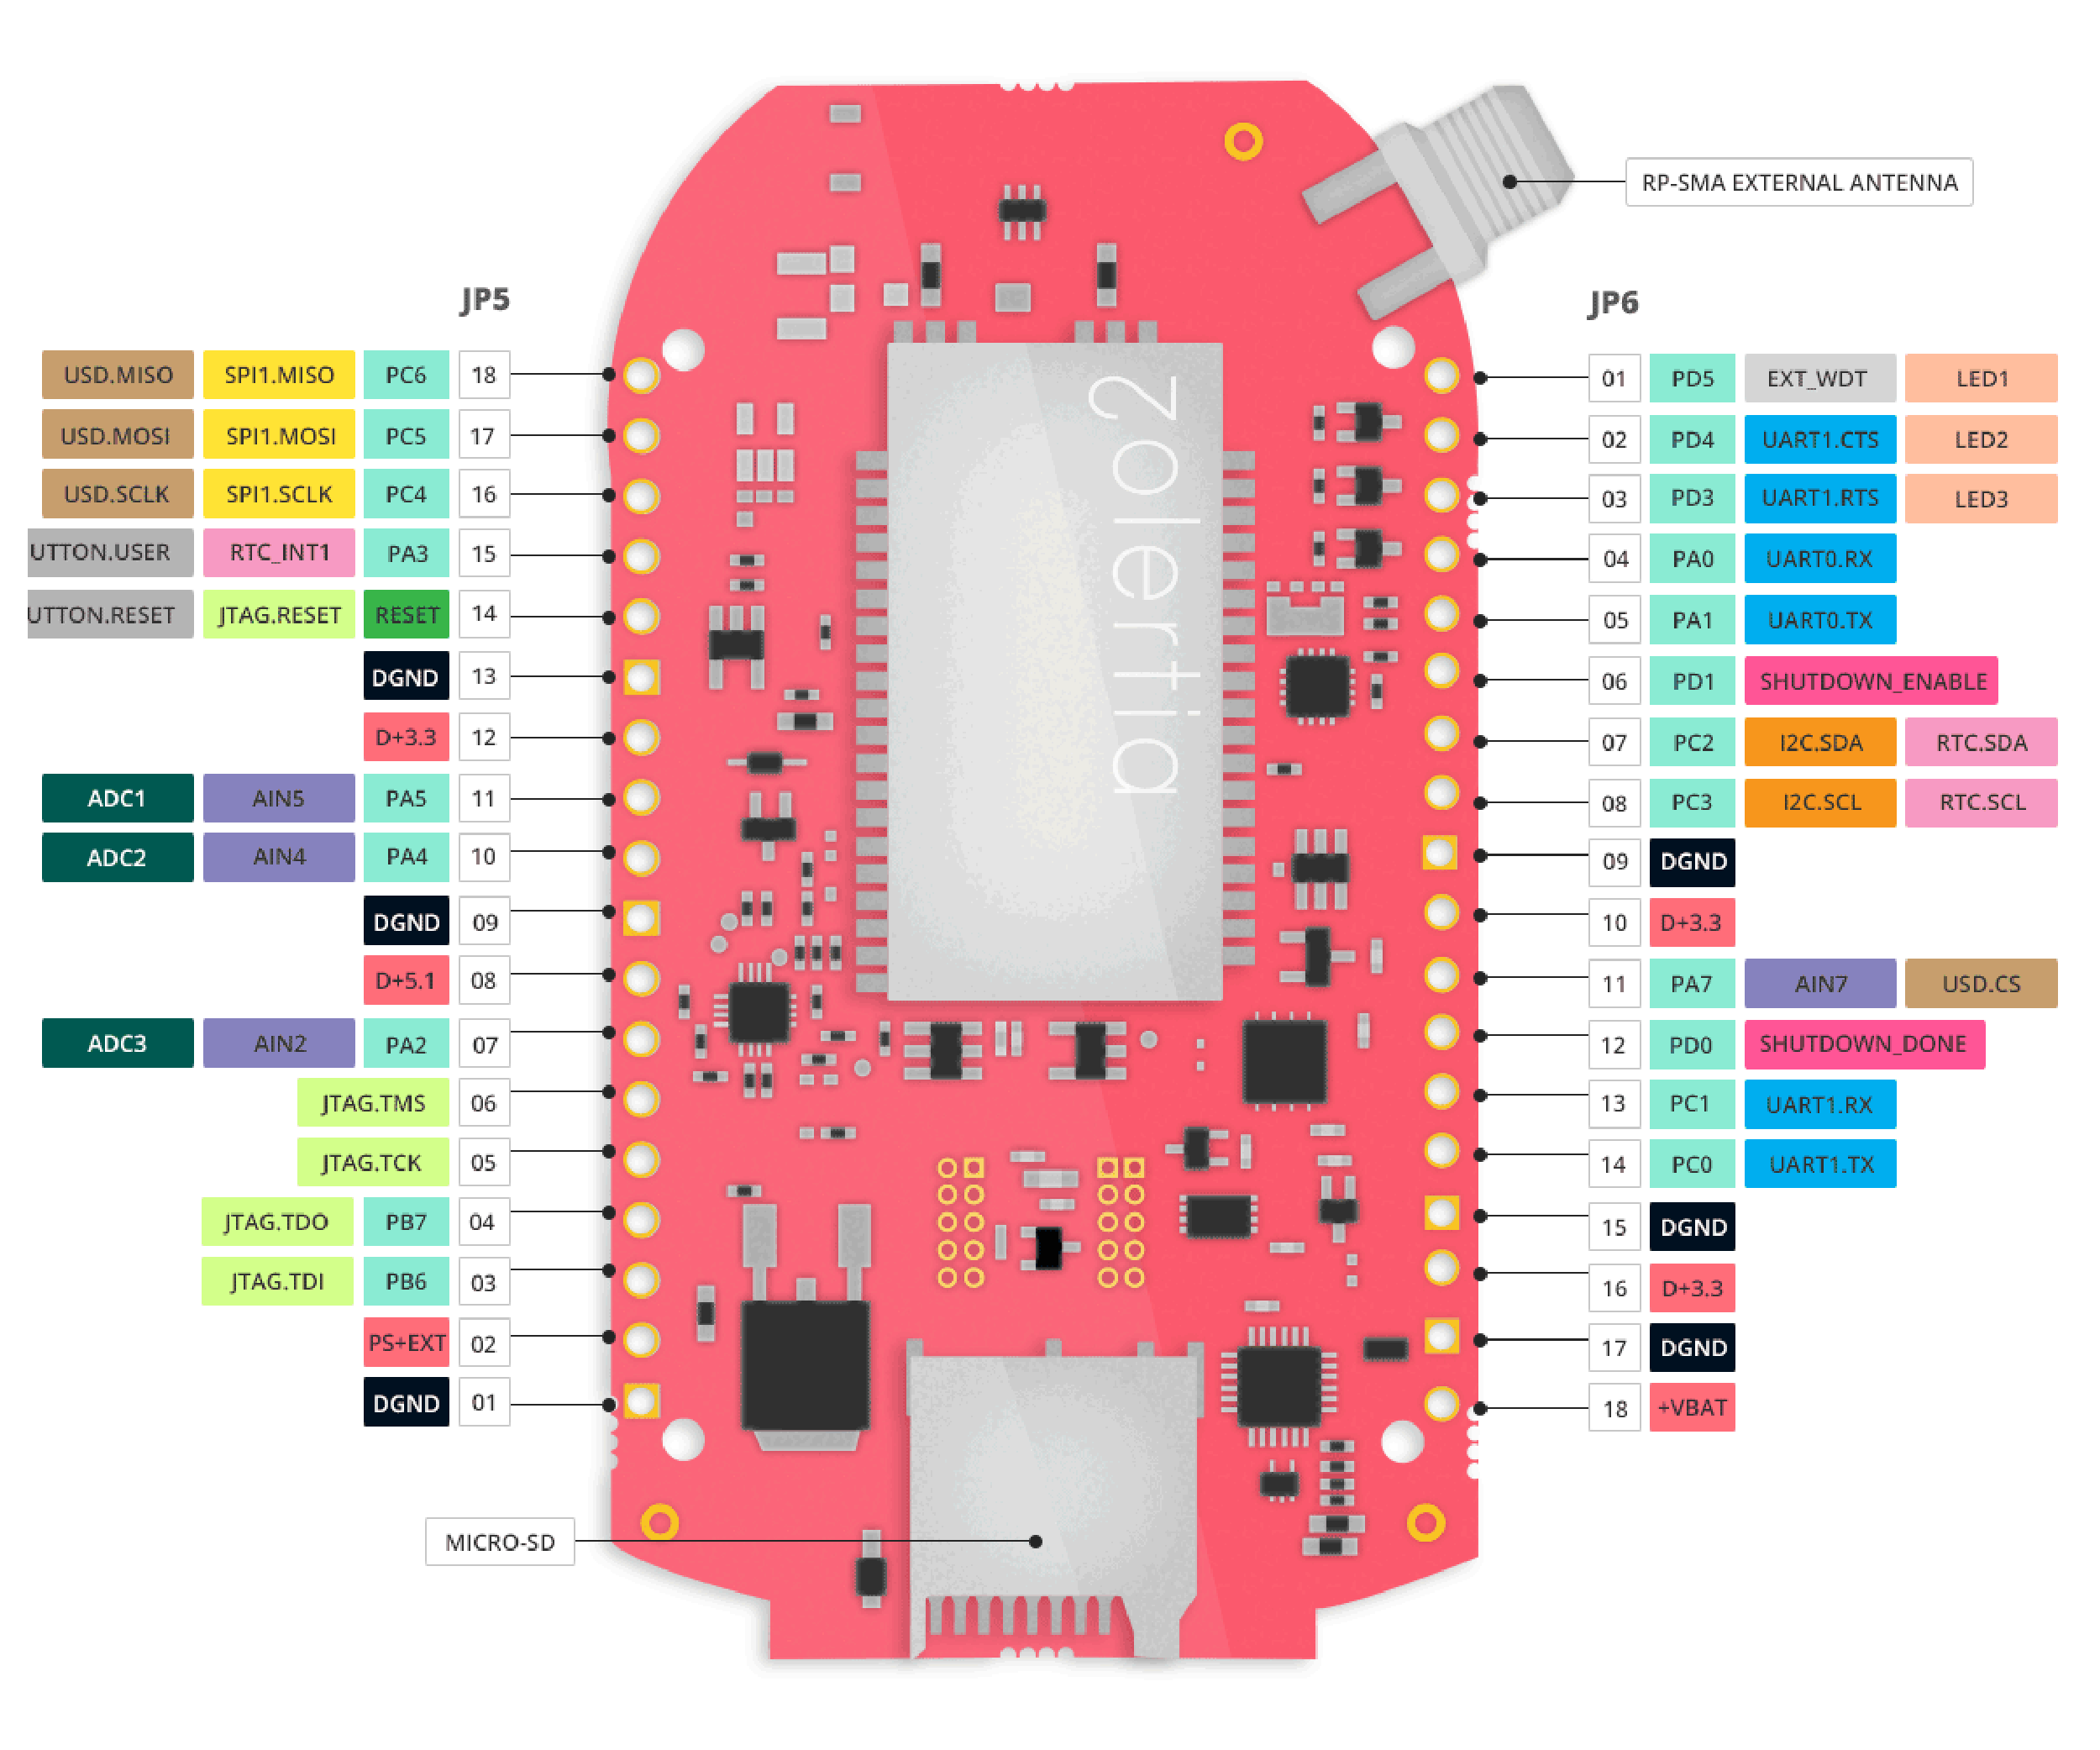
\includegraphics[width=1\textwidth]{images/reva-pins.pdf}
  \subcaption[first caption]{Rev. A}\label{fig:revapins}
\end{minipage}
\begin{minipage}{0.5\textwidth}
  \centering
  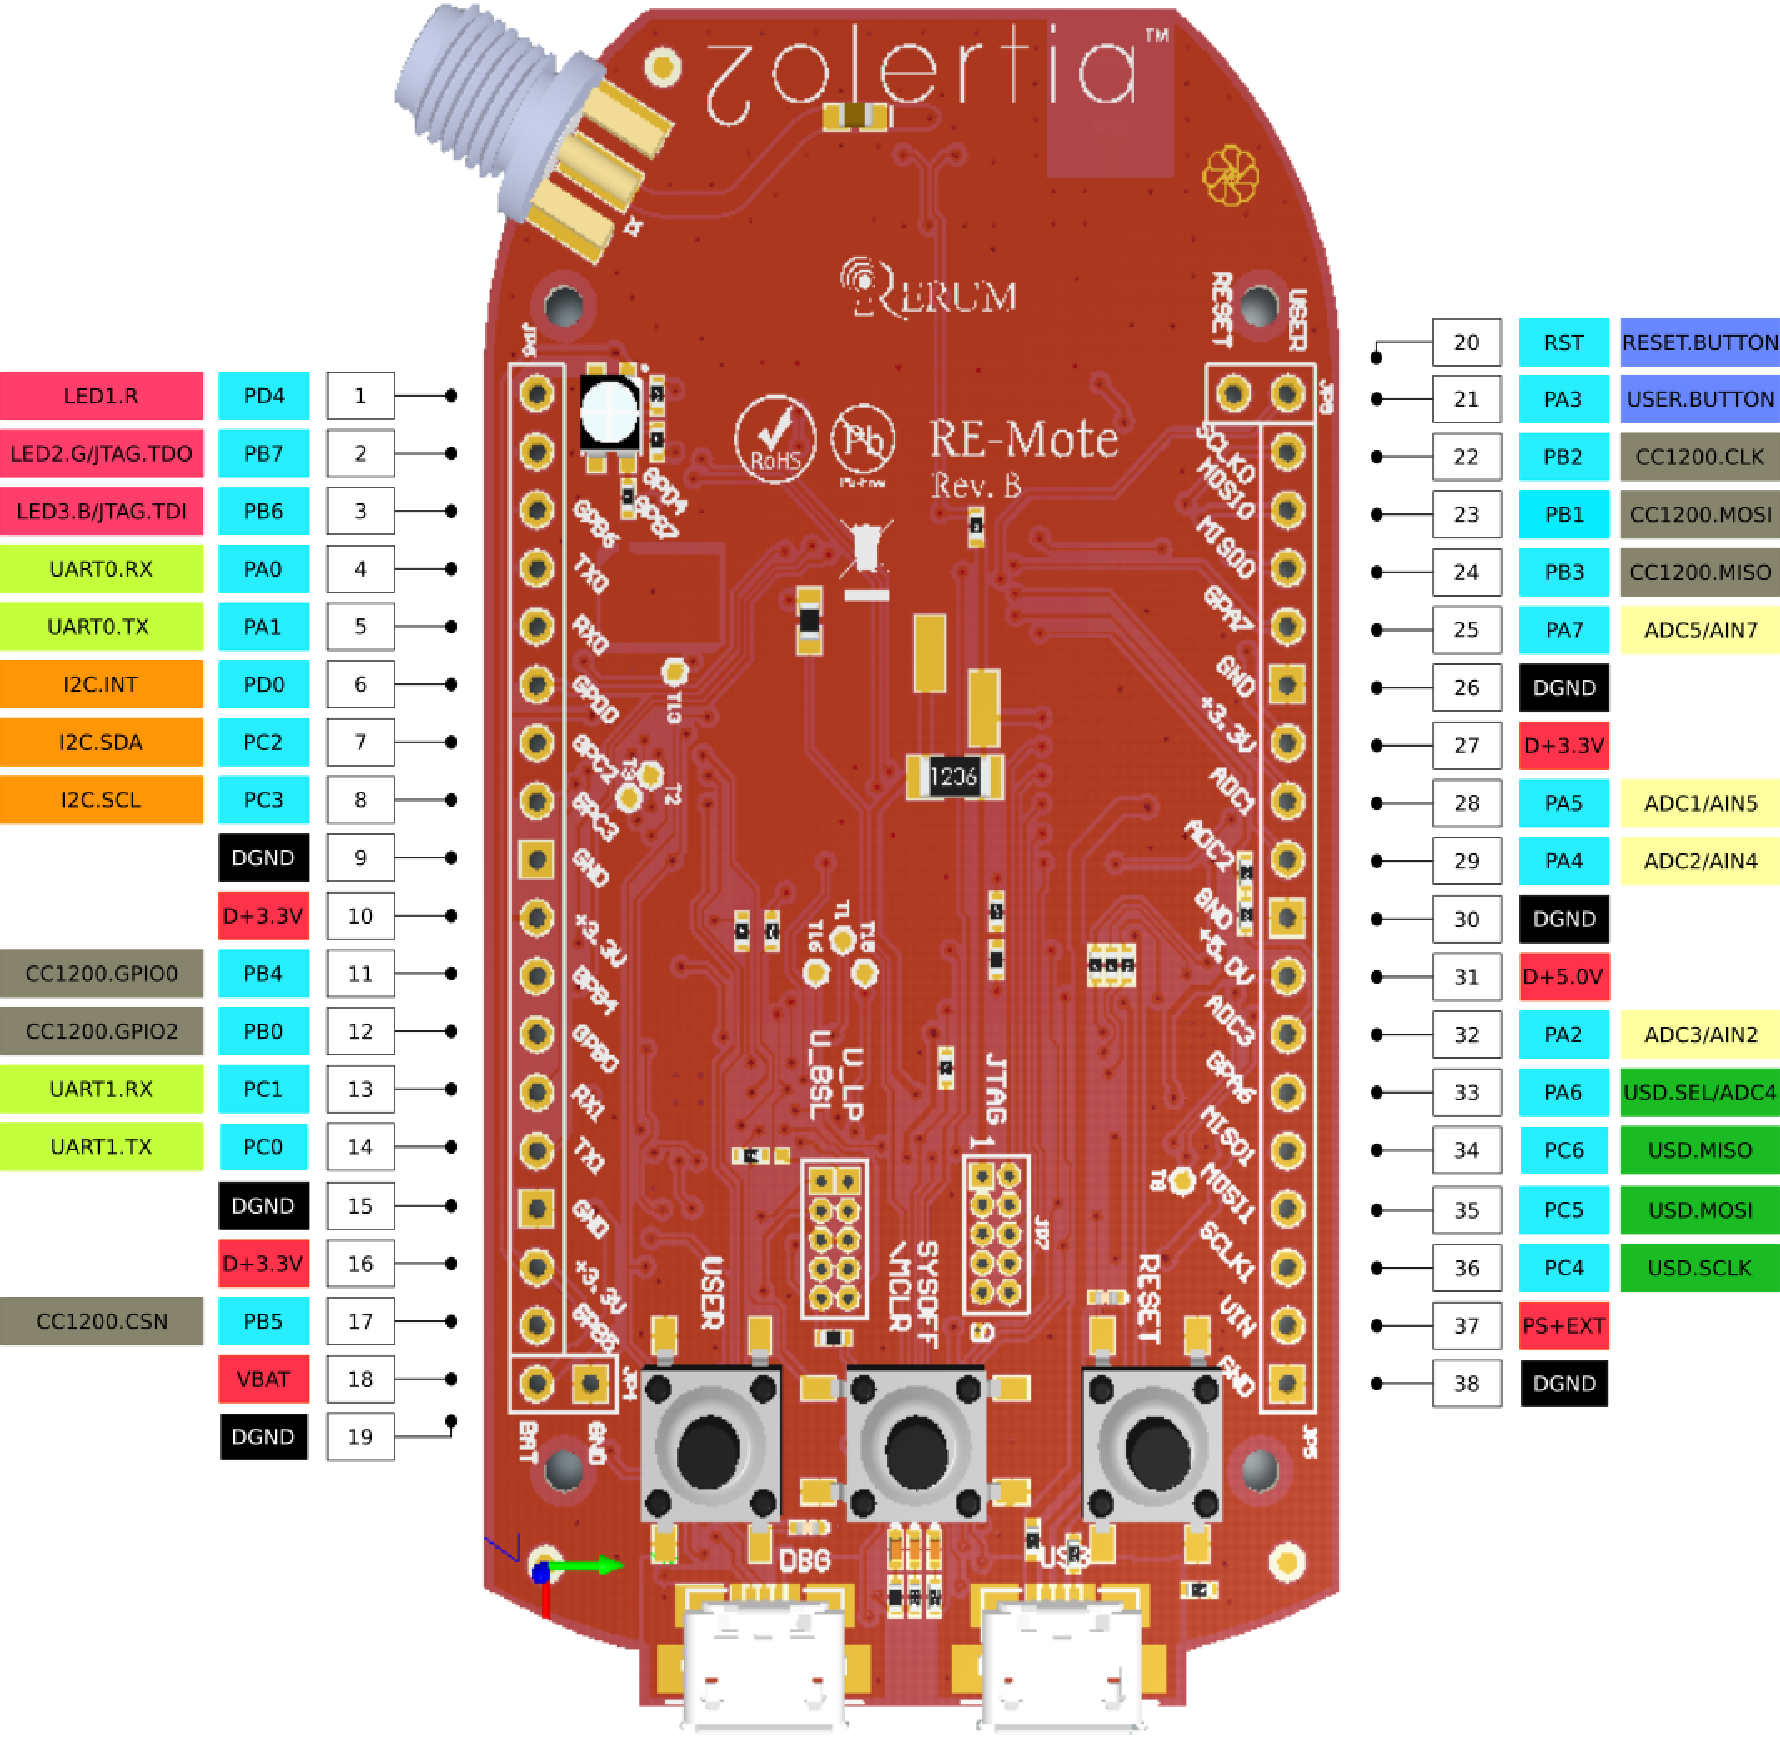
\includegraphics[width=1\textwidth]{images/revb-pins.pdf}
  \subcaption[second caption]{Rev. B}\label{fig:revbpins}
\end{minipage}
\caption{Pin-outs of Zolertia RE-Mote}
\end{figure}

\begin{figure}
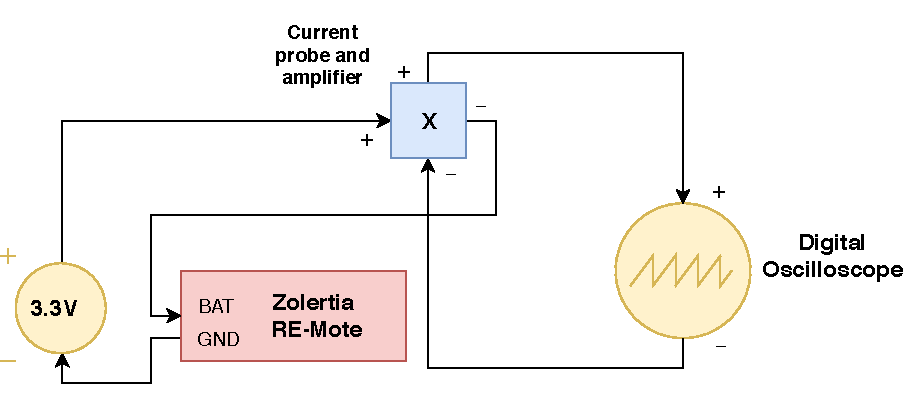
\includegraphics[width=1\textwidth]{images/circuit.pdf}
\caption{\label{fig:circuit}Circuit setup for reading current measurements. X represents the current probe and amplifier arrangement (The Hall effect device)}
\end{figure}

\subsubsection{Uploading code to the RE-Mote}
The objective of this study is to measure current consumption (and thus the energy consumption) of RE-Mote under different scenarios like when,
\begin{itemize}
	\item{Performing computation}
    \item{Sampling a sensor}
    \item{Switching \emph{ON}/\emph{OFF} the Radio}
    \item{Transmitting data}
\end{itemize}
To achieve this, we need to create multiple copies of Contiki OS that tests these different configurations.
The following sub-sections should be repeated for each of the desired configurations. The Contiki OS code should be uploaded to the RE-Mote, each time, after making the desired changes.


\subsubsection{Powering up RE-Mote}
Once the desired code is uploaded to the mote, it should be powered up as follows:
\begin{itemize}
	\item{Use GWINSTEK power supply box and draw 2 wires from 0-30V output}
    \item{Set the voltage to 3.3V}
    \item{Short the two wires and adjust current to 0.03A}
    \item{Connect the two leads to a bread-board}
    \item{Draw two male-female jumpers from these location on the bread-board
      and connect them to BAT and GND of RE-Mote}
\end{itemize}
\textbf{NOTE}: You can verify if the device is powered up by burning border-router
        code on the other RE-Mote and check if data is being transmitted. \par
\textbf{TIP}: Soldering some headers on these pins may be useful, if they don't already exist.

\subsubsection{Setting up the current probe}
In order to use the current probe with the Oscilloscope, the following steps should be performed:
\begin{itemize}
	\item{Connect the current probe output to the current amplifier}
    \item{Connect the current amplifier to oscilloscope output}
	\item{Make sure the DSO channel has load resistance of 50ohms}
    \item{Start up the DSO and the current amplifier}
    \item{Close the current probe if notified by the amplifier indicators (\emph{PROBE OPEN})}
    \item{Press \emph{PROBE DEGAUSS AUTOBALANCE}, to set DC offset to 0}
\end{itemize}
\textbf{CAUTION}: Make sure the current probe is not connected to any circuit
\begin{itemize}
	\item{The DC offset should now be zero, showing that the current probe is de-Gaussed}
\end{itemize}

\subsubsection{Taking measurements}
Follow these steps to take current measurements using the circuit setup:
\linebreak
\linebreak
\textbf{CAUTION}: Use the current probe only after auto-balancing or measurements will be erroneous
\begin{itemize}
    \item{Open the current probe by sliding the switch on it's body}
    \item{Place the wire, going to the device, in the loop, taking care that the 
      arrow points to the direction of flowing current}
\end{itemize}
\textbf{CAUTION}: Do this before powering the device
\begin{itemize}
    \item{Measure the current waveform on the DSO}
\end{itemize}
\textbf{TIP}: You may want to adjust scaling in X and Y

\subsubsection{Saving the waveform}
\begin{itemize}
	\item{Stop the waveform by pressing \emph{Run}/\emph{Stop} button on the DSO}
    \item{Adjust the cursor positions to cover the full width of the data}
    \item{Click on the \emph{File} menu}
    \item{Under \emph{Select for Export} choose \emph{Waveform(data)}}
    \item{Now again click on \emph{File} and then \emph{Export}}
    \item{Save the .dat file in a convenient location}
\end{itemize}

\section{Results and interpretation}
  Temporal plots of current consumption of a Zolertia RE-Mote REV-A and REV-B motes were obtained and the following key observations were made. More accurate results are presented in the plots that follow:
\begin{enumerate}
    \item{Zolertia RE-Mote Rev-B motes consume about 1mA lesser current than Rev-A motes.}
    \item{Power consumption of RE-Mote configured with ContikiMAC duty cycling is about 9 times lesser than without duty cycling}
    \item{Sampling an ADC pin connected to AlphaSense $SO_2$-B4 gas sensors gives a 1mA increase in current consumption}
\end{enumerate}

\paragraph{}
The plots from Fig. \ref{fig:reva-rdcs} to Fig. \ref{fig:revb-tx} show the current consumption of the Zolertia RE-Mote module under various operational conditions.

\paragraph{}
Fig. \ref{fig:reva-rdcs} shows the comparison of current consumption under different Duty cycling mechanisms. If the Radio driver is switched off using the function NETSTACK\_RADIO.off(0) in Contiki, the average current consumed is around 12mA. Contiki MAC duty cycling has a baseline current consumption of about 5mA, while it shoots up to about 30mA when no duty cycling mechanism is used.
\begin{figure}[H]
  \centering
  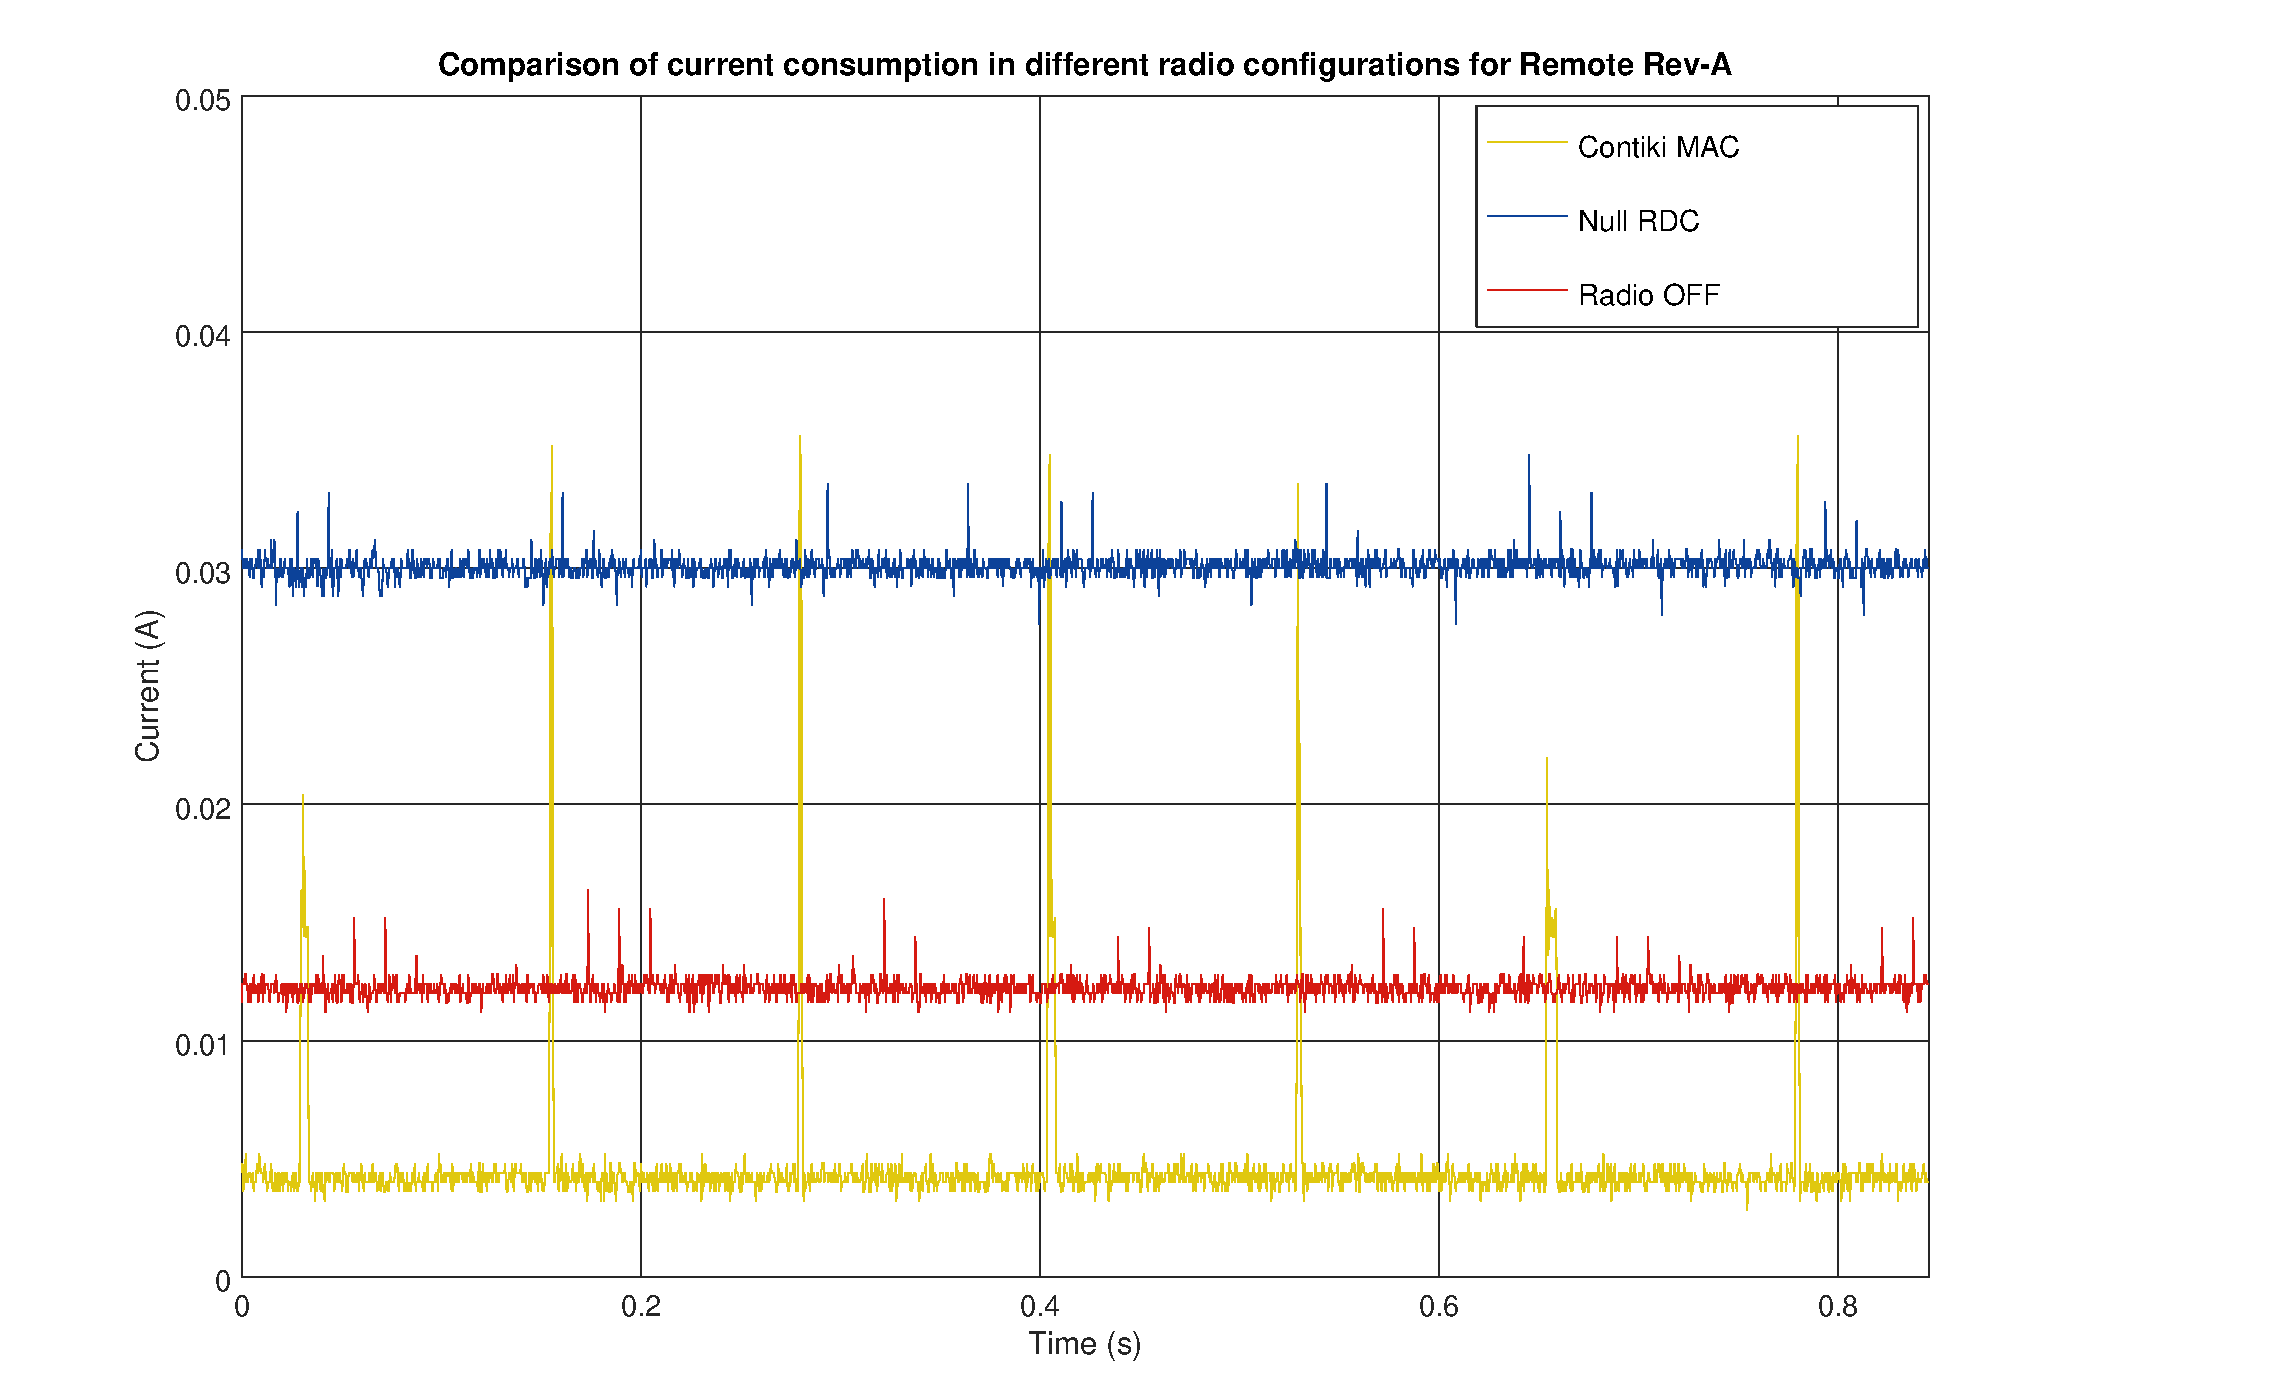
\includegraphics[width=1.0\textwidth]{plots/reva-rdc.eps}
  \caption{\label{fig:reva-rdcs}RE-Mote Revision-A Radio Duty Cycling comparison}
\end{figure}

\paragraph{}
Fig. \ref{fig:revb-rdcs} shows a similar comparison plot for RE-Mote Revision B. The plot is almost identical to Fig. \ref{fig:reva-rdcs} with the exception that each plot shows a drop in current consumption by around 1mA.
\begin{figure}[H]
  \centering
  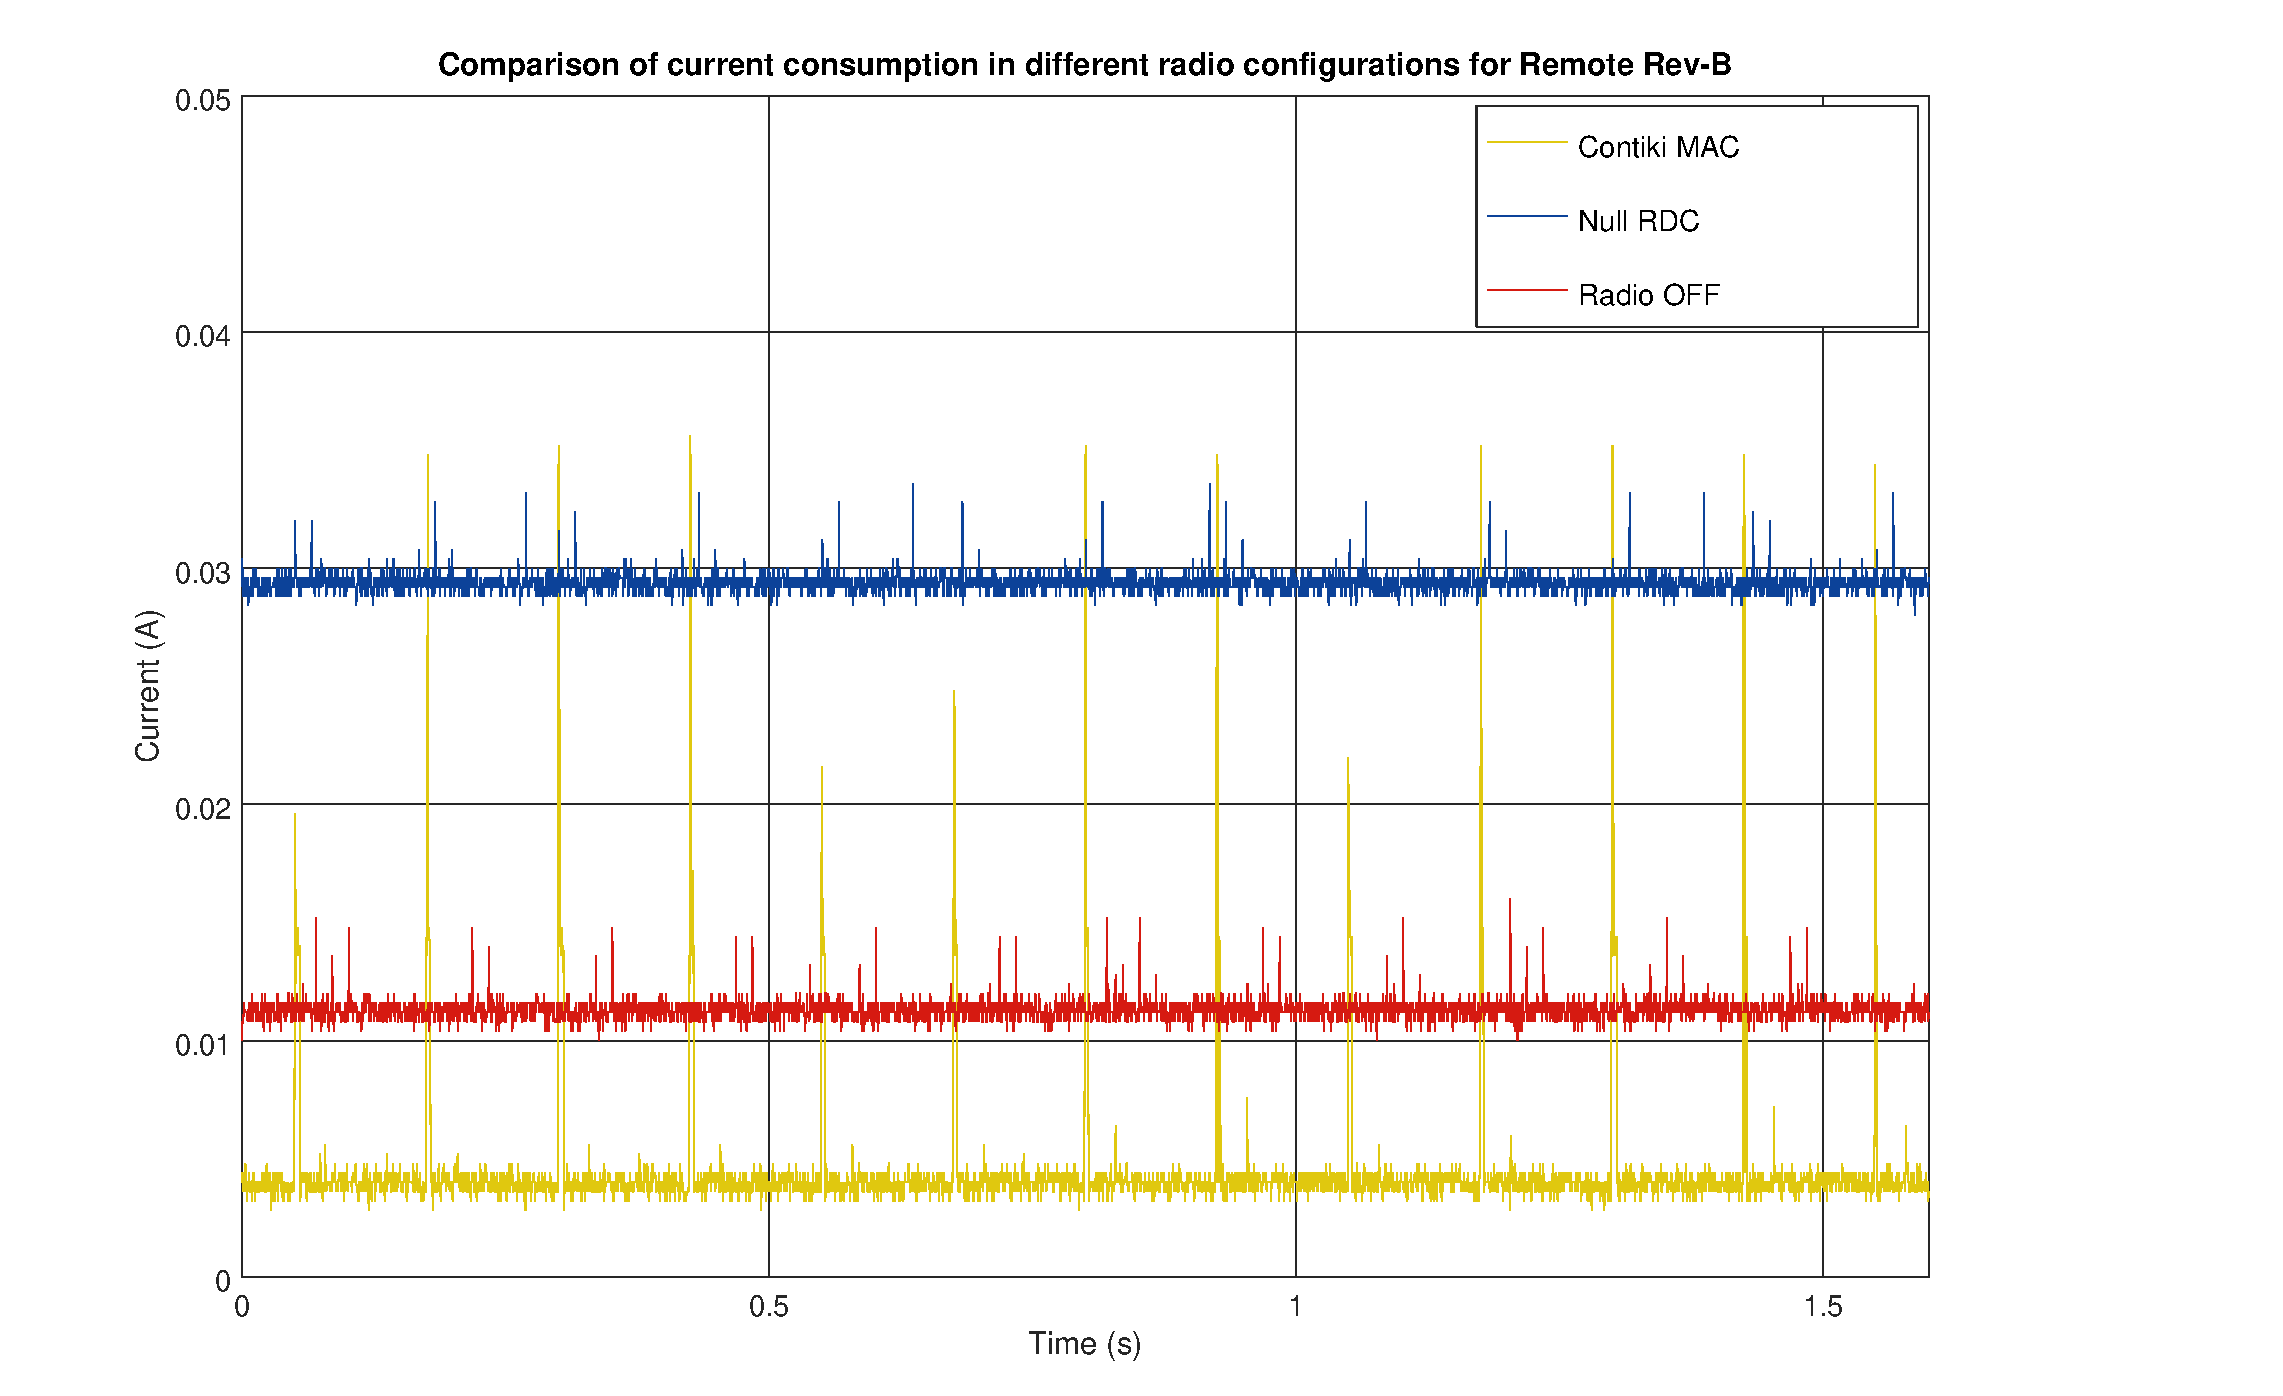
\includegraphics[width=1.0\textwidth]{plots/revb-rdc.eps}
  \caption{\label{fig:revb-rdcs}RE-Mote Revision-B Radio Duty Cycling comparison}
\end{figure}

\paragraph{}
Fig. \ref{fig:revb-sensor} is a plot comparing the current consumption levels on the Rev. B mote when an Analog gas sensor, AlphaSense $SO_2$-B4 is connected to one of the ADC pins of the mote. It is observed that merely powering the sensor through the mote increases the current consumption by about 2mA, and sampling the sensor (reading and converting the received ADC value) leads to a brief surge due to computation.
\begin{figure}[H]
  \centering
  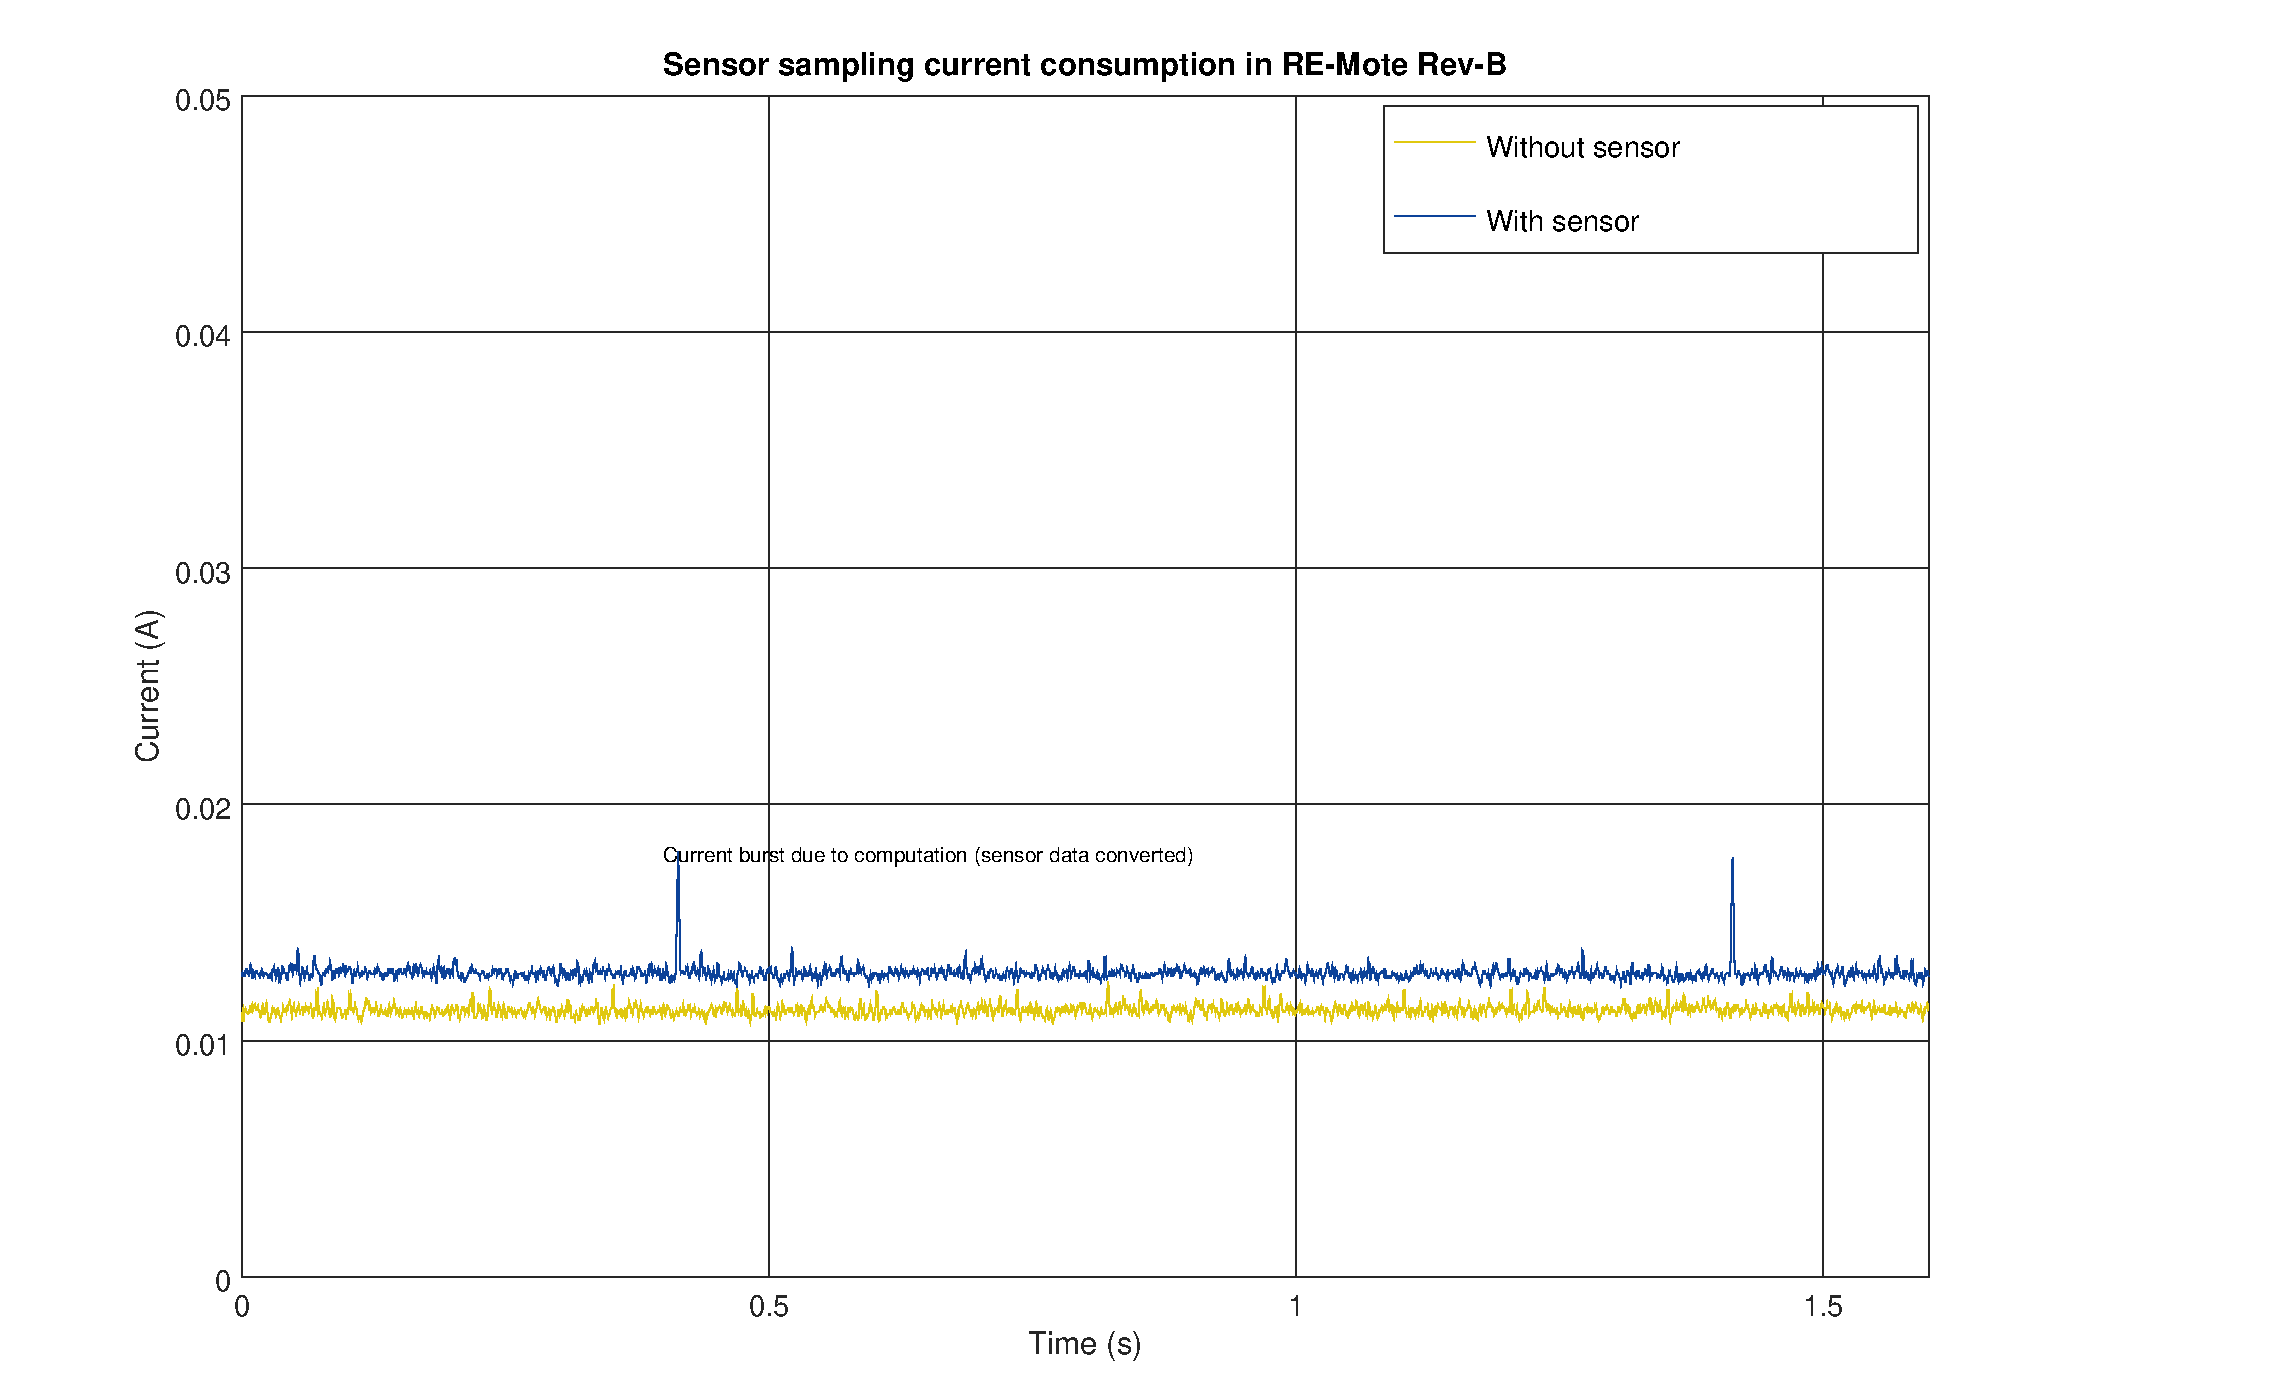
\includegraphics[width=1.0\textwidth]{plots/sensor-onoff-comparison.eps}
  \caption{\label{fig:revb-sensor}RE-Mote Revision-B Sampling ADC pin connected to AlphaSense $SO_2$-B4 sensor}
\end{figure}

\paragraph{}
In Fig. \ref{fig:revb-cmpt}, we notice that the current consumption increases by about 2mA. Here the computation performed is addition.
\begin{figure}[H]
  \centering
  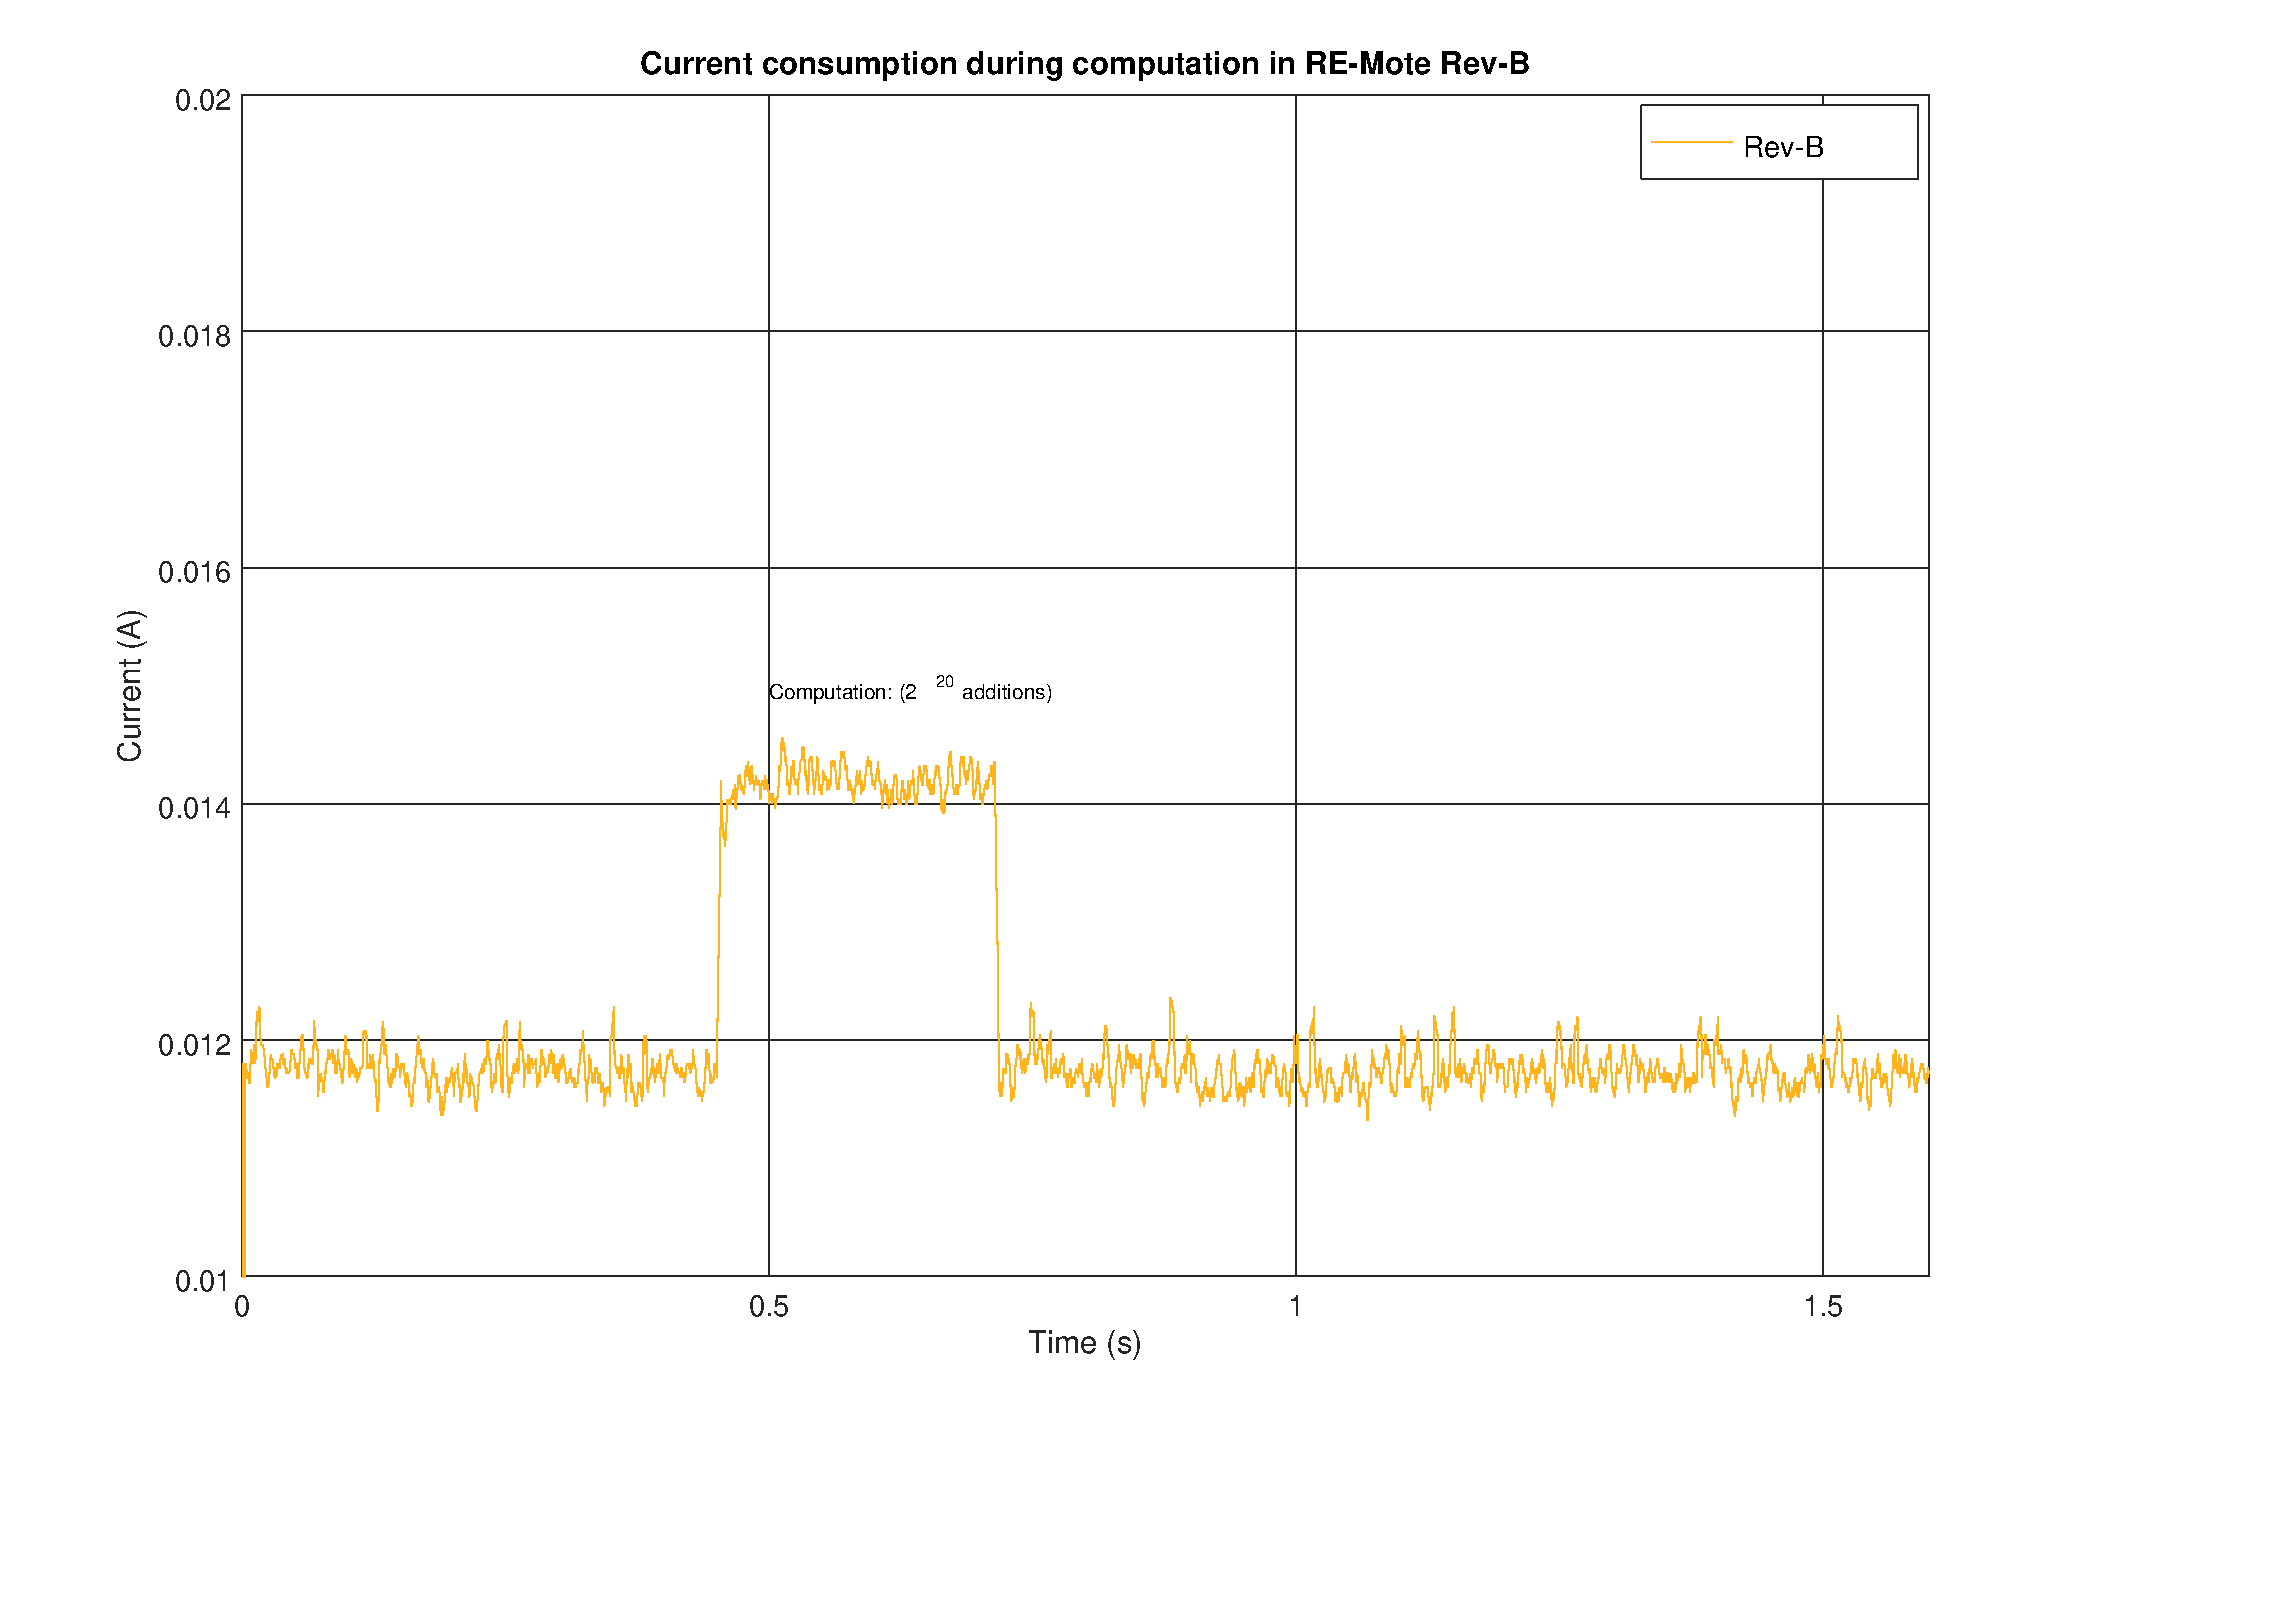
\includegraphics[width=1.0\textwidth]{plots/comp-revb.eps}
  \caption{\label{fig:revb-cmpt}RE-Mote Revision-B Computation of $2^20$ additions}
\end{figure}

\paragraph{}
Fig. \ref{fig:revb-tx} shows the increase in current consumption when transmitting a packet. Scenarios where Duty cycling in on and off are shown in different colours for comparison. It can be noted that the increase in current consumption is about 5mA without duty cycling and is about 12mA with Contiki MAC duty cycling. This is most likely because in ContikiMAC duty cycling, the mote needs an extra 7mA to wake up from sleep state.
\begin{figure}[H]
  \centering
  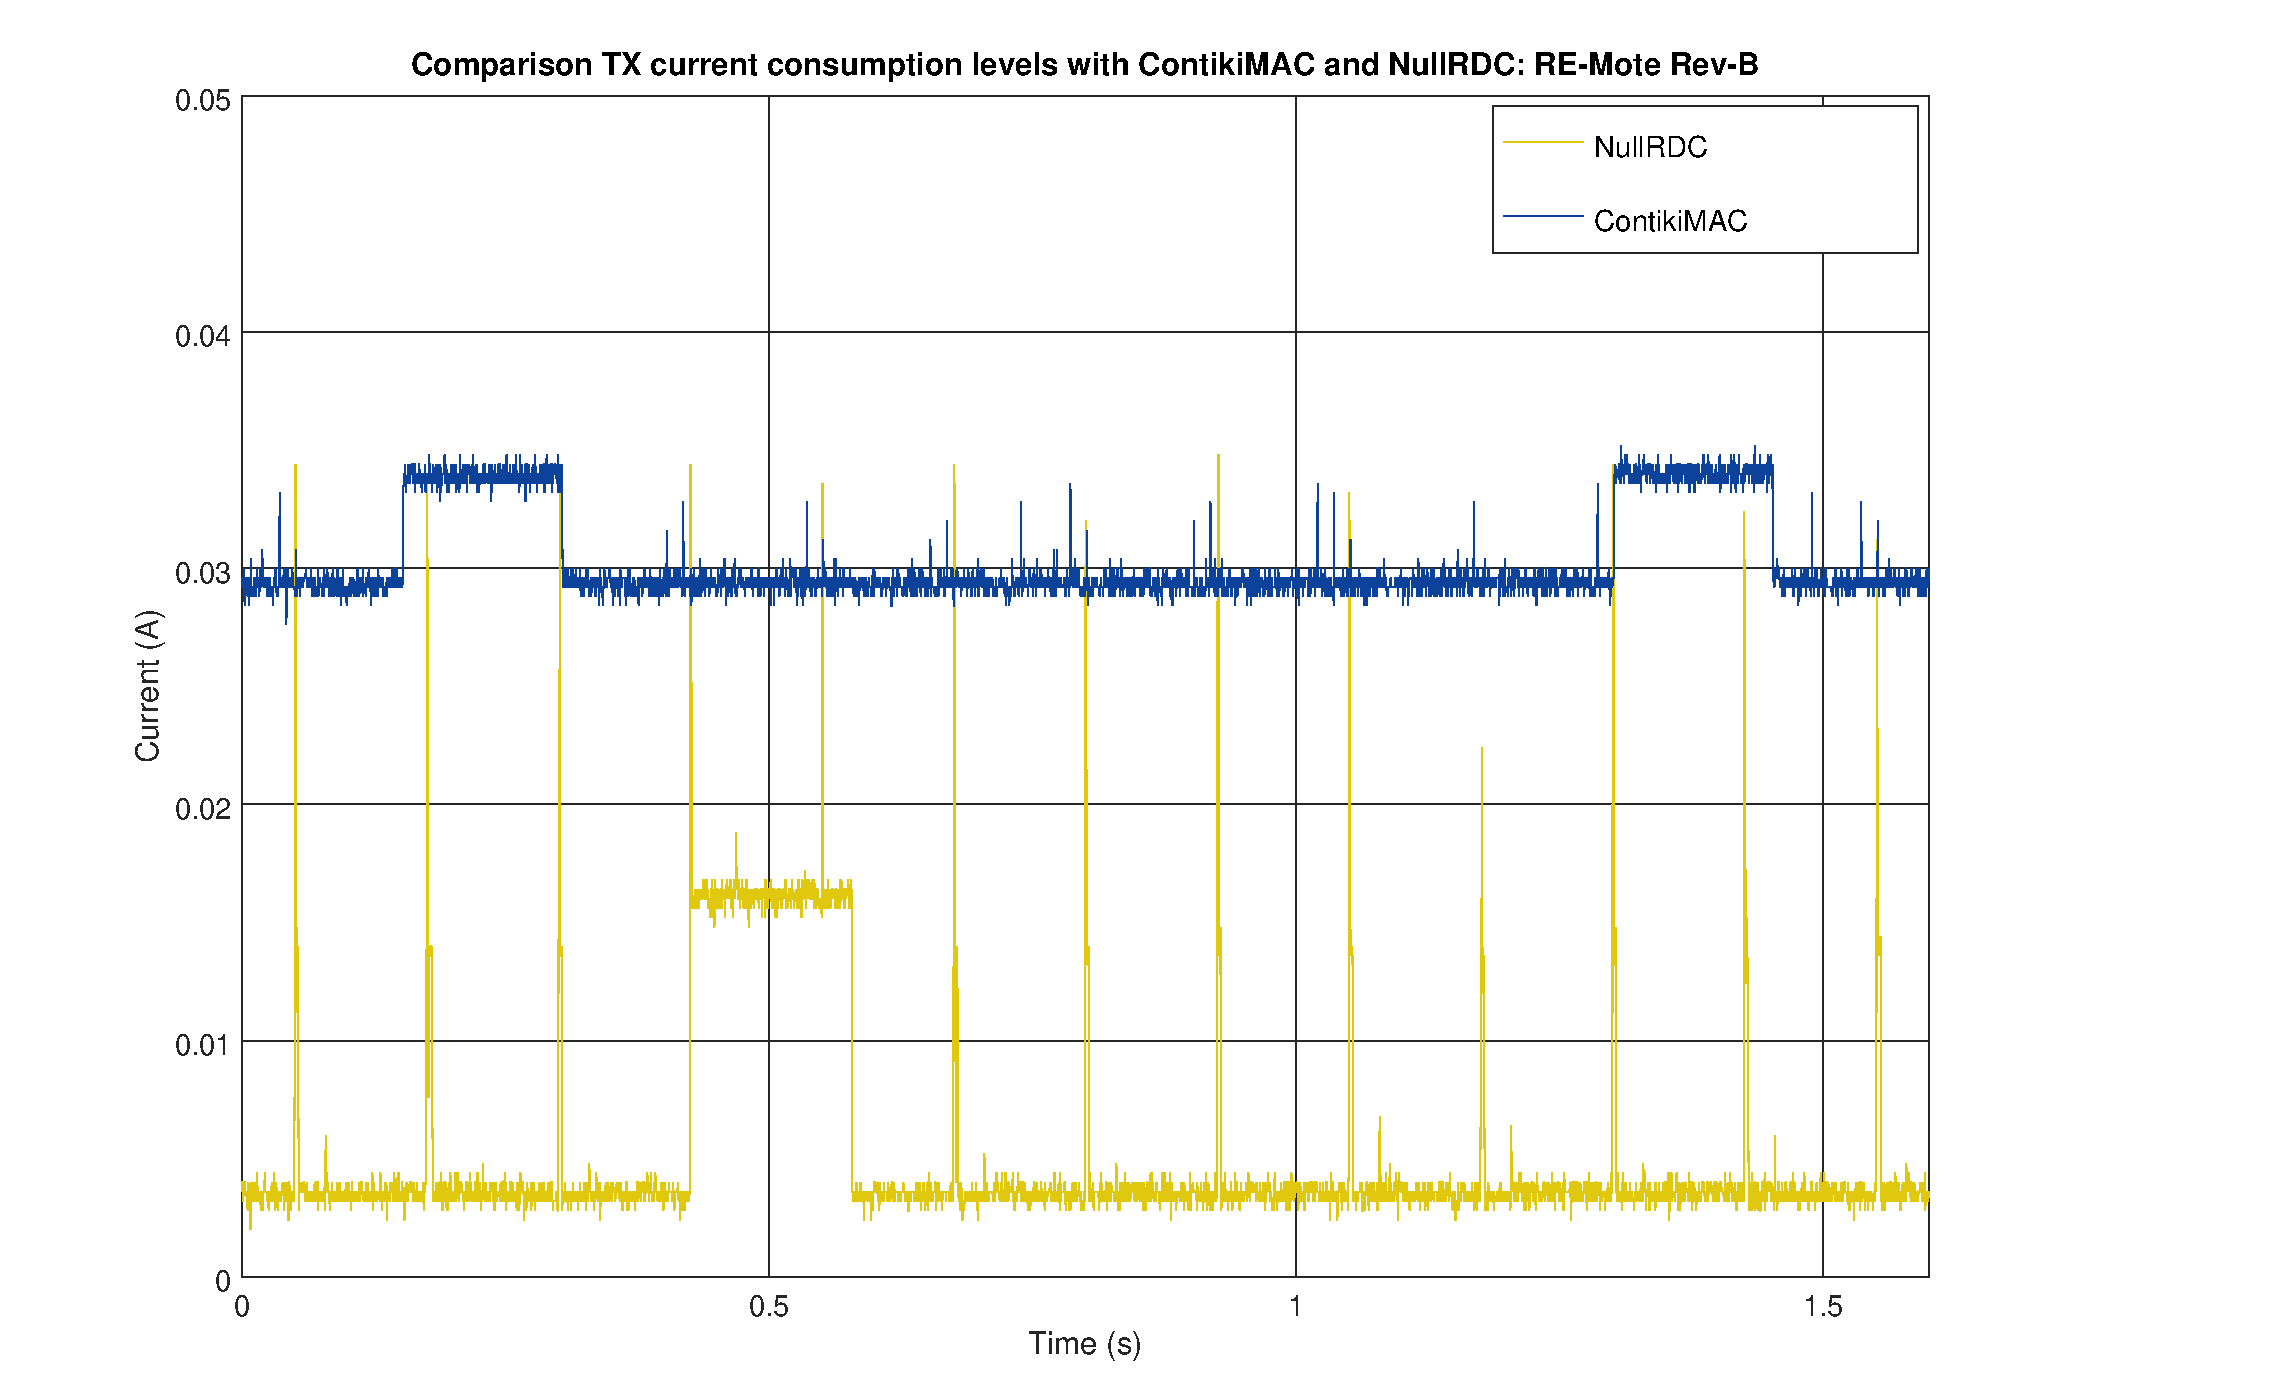
\includegraphics[width=1.0\textwidth]{plots/tx_comparison_revb.eps}
  \caption{\label{fig:revb-tx}RE-Mote Revision-B Comparing transmission with and without Radio Duty Cycling}
\end{figure}

\section{Conclusion}
Power profiling experiments, such as the one presented above, can give a detailed understanding of how to optimize power budget in a large scale IoT deployment. This can directly impact not only the budget of a deployment, but also the battery life of the motes used. It is clear from the above experiments that Radio Duty Cycling plays an important role in optimizing energy consumption. Moreover the number of transmissions, and thus the number of exchanges in a large scale network, should be minimized if one desires to optimize energy consumption.

\begin{thebibliography}{9}
\bibitem{remote}
  Zolertia RE-Mote wiki, https://github.com/Zolertia/Resources/wiki/RE-Mote
\bibitem{ieee802154}
  J. A. Gutierrez, M. Naeve, E. Callaway, M. Bourgeois, V. Mitter and B. Heile, "IEEE 802.15.4: a developing standard for low-power low-cost wireless personal area networks," in IEEE Network, vol. 15, no. 5, pp. 12-19, Sept.-Oct. 2001.
\bibitem{contiki}
  A. Dunkels, B. Gronvall and T. Voigt, "Contiki - a lightweight and flexible operating system for tiny networked sensors," 29th Annual IEEE International Conference on Local Computer Networks, 2004, pp. 455-462.
\bibitem{contikimac}
  A. Dunkels, "The ContikiMAC Radio Duty Cycling Protocol", SICS Technical Report T2011:13, ISSN 1100-3154
\bibitem{git-repo}
  GitHub repository for Power profiling RE-Mote platform: \url{https://www.github.com/srijith1996/zolertia-remote-power-profile}

\end{thebibliography}
\end{document}
